% Version 3.1 December 2024
% See section 11 of the User Manual for version history
%
%%%%%%%%%%%%%%%%%%%%%%%%%%%%%%%%%%%%%%%%%%%%%%%%%%%%%%%%%%%%%%%%%%%%%%
%%                                 %%
%% Please do not use \input{...} to include other tex files.    %%
%% Submit your LaTeX manuscript as one .tex document.       %%
%%                                 %%
%% All additional figures and files should be attached       %%
%% separately and not embedded in the \TeX\ document itself.    %%
%%                                 %%
%%%%%%%%%%%%%%%%%%%%%%%%%%%%%%%%%%%%%%%%%%%%%%%%%%%%%%%%%%%%%%%%%%%%%

\documentclass[pdflatex,iicol,sn-mathphys-ay]{sn-jnl}

%%%% Standard Packages
\usepackage{graphicx}%
\usepackage{multirow}%
\usepackage{amsmath,amssymb,amsfonts}%
\usepackage{amsthm}%
\usepackage{mathrsfs}%
\usepackage[title]{appendix}%
\usepackage{xcolor}%
\usepackage{textcomp}%
\usepackage{manyfoot}%
\usepackage{booktabs}%
\usepackage{algorithm}%
\usepackage{algorithmicx}%
\usepackage{algpseudocode}%
\usepackage{listings}%
\usepackage{rotating}%
\usepackage{tikz}
\usepackage{xurl}
\usetikzlibrary{shapes.geometric, arrows.meta, positioning, calc, fit, backgrounds}

\theoremstyle{thmstyleone}%
\newtheorem{theorem}{Theorem}%
\newtheorem{proposition}[theorem]{Proposition}%

\theoremstyle{thmstyletwo}%
\newtheorem{example}{Example}%
\newtheorem{remark}{Remark}%

\theoremstyle{thmstylethree}%
\newtheorem{definition}{Definition}%

\raggedbottom

\begin{document}

\title[Explainable Hotel Cancellation Prediction Models]{Explainable Hotel Booking Cancellation Prediction Models: Towards Trustworthy Survival Analysis in Hospitality}

\author*[1]{\fnm{Mustafa} \sur{Cavus}}\email{mustafacavus@eskisehir.edu.tr}
\affil[1]{\orgname{Eskisehir Technical University}, \orgdiv{Department of Statistics}, \postcode{26555}, \city{Eskisehir}, \country{Türkiye}}

\abstract{Hotel booking cancellations impose significant operational uncertainty and financial losses on revenue management systems, traditionally addressed through static binary classification. While binary classifiers predict whether a reservation will ultimately be canceled, they inherently neglect the temporal dimension, specifically \textit{when} cancellation occurs, and introduce systematic predictive bias when applied to right-censored reservation records. This study introduces an explainable time-to-event modeling framework that directly addresses these limitations using a large-scale empirical dataset of resort and city hotel reservations with verified timestamps. We benchmark diverse survival algorithms spanning semi-parametric hazard formulations, penalized regression, and non-parametric machine learning ensembles. The experimental evaluation incorporates a stratified train-test split, cross-validation, non-parametric bootstrap resampling, pairwise statistical hypothesis testing, and empirical probability calibration curves across multiple operational horizons. Our findings demonstrate a critical trade-off: while standard Random Survival Forests maximize discriminative risk ranking, Oblique Random Survival Forests achieve superior probability calibration and closely align with empirical Kaplan-Meier event rates across continuous lead-time intervals. Furthermore, we deploy continuous time-dependent XAI tools, namely Survival Permutation Feature Importance and Partial Dependence Survival Profiles, to audit the predictive behavior of survival models. These explanations reveal non-linear, time-varying risk trajectories, showing that lead time and deposit policies dominate early-stage vulnerability, while highlighting structural anomalies where non-refundable rates exhibit elevated cancellation rates due to speculative block bookings. The proposed framework provides hospitality enterprises with an auditable, trustworthy, and ethically grounded decision-support foundation that mitigates consumer insecurity from aggressive overbooking, prevents algorithmic misclassifications, and aligns digital transformation with responsible governance.}

\keywords{hotel booking cancellation, XAI, survival analysis, random survival forests, revenue management, trustworthy AI}

\maketitle

%%%%%%%%%%%%%%%%%%%%%%%%%%%%%%%%%%%%%%%%%%%%%%%%%%%
\section{Introduction}
\label{sec:introduction}

In the tourism sector, demand forecasting stands as a foundational pillar for strategic capacity management \citep{antonio2017predicting}, resource allocation, and dynamic pricing optimization \citep{ampountolas2025predicting}. Beyond its operational utility, predictive modeling in hospitality functions as a mechanism that converts raw transactional data into strategic intelligence, enabling industry stakeholders and policymakers to formulate competitive strategies and narrow the structural gap between projected supply and realized demand \citep{herrera2024machine}. Unlike traditional inventory-based businesses, hotel room reservations represent highly perishable services where an unallocated room on any given calendar night results in an absolute loss of potential revenue \citep{antonio2019big}, meaning hotels cannot recover the value of unsold capacity once a night passes \citep{mir2026decoding}. Consequently, revenue management departments rely on predictive analytics to maintain occupancy levels \citep{yoo2024predicting} and capture maximum market value through dynamic inventory controls \citep{liu2025explainable}. However, the accuracy of short-term demand signals is fundamentally distorted by hotel booking cancellations. These cancellations compromise forecasting reliability \citep{liu2023hospitality, luo2025hotel} and account for operational losses estimated at approximately 20\% of hotel revenues \citep{sierag2015revenue, falk2018modelling}.

The widespread adoption of online travel agencies and digital booking channels has structurally altered consumer behavior by introducing high price transparency and lowering the transactional barriers to canceling previously confirmed reservations. Prospective travelers frequently exhibit opportunistic behaviors, using flexible policies to secure multiple alternatives \citep{chen2023prediction} or engaging in intertemporal arbitrage by rebooking when lower rates emerge \citep{mir2026decoding} closer to their scheduled arrival date \citep{ampountolas2025predicting}. This phenomenon intensified markedly in the aftermath of the COVID-19 pandemic, during which major online travel platforms introduced permanently flexible cancellation terms to restore consumer confidence. As a structural legacy, these liberalized refund policies normalized last-minute reservation modifications and cultivated a segment of highly rate-sensitive travelers who treat booked reservations as provisional options rather than binding commitments. The consequent elevation in baseline cancellation rates, rising from pre-pandemic averages of 20–30\% to post-pandemic levels exceeding 40\% in some European urban markets, has substantially amplified the operational burden placed on revenue management teams \citep{mir2026decoding}. To hedge against this persistent operational risk, hotels conventionally enforce restrictive, non-refundable penalty windows \citep{yang2024predicting} or deploy overbooking quotas \citep{antonio2017predicting}. Nevertheless, these traditional practices often yield negative externalities, such as eroding customer satisfaction, triggering high relocation costs, and damaging the brand reputation of the property in competitive digital ecosystems \citep{falk2018modelling}. To circumvent the adverse consequences of blanket restrictions, revenue managers increasingly rely on predictive models to estimate individual booking cancellation probabilities, enabling personalized retention actions and granular capacity controls \citep{antonio2017predicting, liu2023hospitality, talal2025hotel}.

Within this context, positioning the cancellation problem correctly within the predictive modeling architecture is crucial. Because reservation commitments evolve dynamically as the arrival date approaches, effective revenue management requires continuous monitoring of cancellation hazards rather than static risk snapshots. Nevertheless, traditional hotel booking cancellation prediction studies generally frame the task as static binary classification, focusing solely on predicting whether a booking will ultimately be canceled. This conventional framing inherently ignores the temporal progression of cancellation risks and introduces systematic predictive bias when applied to reservations that remain active in the system with future check-in dates. In historical reservation cohorts, such incomplete observations constitute right-censored data that require time-to-event approaches rather than static classification \citep{kleinbaum2012survival, langbein2025interpretable}. As conceptually illustrated in Figure~\ref{fig:motivation}, survival analysis models resolve this fundamental bias by mathematically integrating right-censored records into the likelihood framework \citep{kovalev2020survlime, langbein2025interpretable}. Crucially, by estimating both the continuous survival trajectory and the instantaneous hazard rate over time, time-to-event modeling provides hospitality enterprises with an actionable roadmap. Predicting precisely \textit{when} an attrition event is most probable enables revenue management systems to dynamically adjust overbooking quotas, determine optimal re-marketing windows for perishable rooms before demand decays \citep{mir2026decoding}, and deploy proactive retention interventions at minimal mitigation cost \citep{antonio2017predicting, ampountolas2025predicting}.

To illustrate the practical stakes of this temporal distinction, consider two reservations with identical covariates, same lead time, same booking channel, same room type, but made at different points in the booking window. A static binary classifier would assign identical cancellation probabilities to both. A survival model, in contrast, recognizes that the reservation closer to its check-in date has already survived a portion of the high-risk window and assigns it a substantially lower instantaneous hazard. This distinction is operationally critical: a revenue manager relying on static probabilities would over-allocate retention resources to low-risk bookings while missing the narrow re-marketing window for high-risk ones. The ability to model \textit{when} risk peaks, not merely whether it exists, transforms cancellation prediction from a classification exercise into a continuous decision-support instrument.

Despite these evident benefits, the practical adoption of sophisticated machine learning survival algorithms, such as Random Survival Forests, gradient-boosted survival trees, and regularized Cox ensembles, is substantially hindered by their \textit{black-box} complexity. As the digital transformation of hospitality accelerates, enterprises increasingly delegate high-stakes forecasting, inventory rationing, and pricing decisions to autonomous algorithmic agents \citep{dwivedi2025artificial}. However, deploying opaque predictive systems generates profound ethical challenges, consumer insecurity, and organizational risks \citep{lin2026developing}. When automated algorithms make unexplainable cancellation forecasts, aggressive overbooking policies frequently lead to guest displacement, eroding consumer trust and brand legitimacy. Recent scholarship highlights that ethical artificial intelligence in tourism is not merely a theoretical aspiration but an operational imperative grounded in transparency, explainability, fairness, and accountability \citep{law2025ethical, meske2022explainable, thiebes2021trustworthy}. In competitive hospitality ecosystems, managers are rightfully reluctant to deploy automated models whose temporal forecasts cannot be interpreted, audited, or aligned with domain logic. While Explainable Artificial Intelligence frameworks have achieved widespread success in explaining static classifiers, explaining time-to-event predictions introduces distinct mathematical challenges due to the continuous and multi-dimensional nature of survival trajectories.

To bridge these critical gaps and operationalize trustworthy AI principles within hospitality management, this paper introduces an end-to-end explainable time-to-event modeling framework. To the best of our knowledge, this is the first study in hospitality revenue management that couples advanced machine learning survival models with continuous, time-dependent global XAI tools. Specifically, this research delivers three principal contributions to literature and practice:
\begin{enumerate}
\item We reframe hotel booking cancellation forecasting as a continuous time-to-event survival analysis problem with verified censoring timestamps, benchmarking diverse survival algorithms with non-parametric bootstrap uncertainty estimates and statistical significance testing, demonstrating that Oblique Random Survival Forests achieve superior probability calibration for operational risk management.
\item We introduce time-dependent XAI methods, specifically Survival Permutation Feature Importance and Partial Dependence Survival Profiles, to the hospitality domain, tracking the evolving marginal impact of reservation attributes over the booking window to reveal compounding price elasticity near arrival and unmask policy-driven structural anomalies.
\item We bridge algorithmic machine learning outputs with actionable decision support for hotel revenue managers, translating transparent and auditable survival curves into dynamic overbooking quotas, optimal room re-marketing windows, and responsible AI governance.
\end{enumerate}

The scale of the economic problem further motivates the methodological shift pursued in this study. Global hotel industry research consistently reports that cancellation rates across European city hotels range between 30\% and 45\%, with platform-mediated bookings through online travel agencies exhibiting rates approaching 50\% in peak seasons \citep{antonio2019big, falk2018modelling}. At these magnitudes, even a marginal improvement in cancellation timing prediction, knowing whether a high-risk booking is likely to cancel in the next seven days versus the next thirty, can translate into millions of euros in recovered revenue through timely room re-marketing and overbooking optimization. The aggregate financial impact underscores why the temporal resolution of cancellation prediction, not merely its directional accuracy, is the operationally decisive modeling challenge.

Furthermore, the literature has not adequately addressed the methodological mismatch between the data-generating process of hotel cancellations and the statistical models conventionally applied to predict them. Hotel cancellations are inherently time-to-event phenomena: each reservation enters a risk window at booking time and exits either through cancellation or check-in arrival. Any model that ignores this risk window, treating the outcome as a fixed binary label rather than a duration-conditional event, implicitly misspecifies the data-generating process and produces estimates that are valid only under assumptions that historical hotel booking data routinely violate. The survival analysis framework adopted in this study is not merely a methodological novelty; it is the statistically correct formulation of the hotel cancellation problem, and the improvements in calibration and temporal resolution documented in our results reflect this underlying correctness.

The remainder of this paper is organized as follows. Section~\ref{sec:related_work} reviews the relevant literature on cancellation prediction, XAI in hospitality, and survival analysis methods. Section~\ref{sec:methodology} formalizes the time-to-event modeling framework and the deployed XAI techniques. Section~\ref{sec:experimental_design} describes the datasets, survival schema construction, and evaluation pipeline. Section~\ref{sec:results} presents and interprets the empirical results across predictive performance and model explanations. Section~\ref{sec:discussion} situates the findings within the broader literature and discusses managerial implications. Section~\ref{sec:conclusion} concludes with limitations and future research directions.

\section{Related Work}
\label{sec:related_work}

The literature on hotel booking cancellation prediction has evolved substantially over the past decade, progressing from classical statistical models to complex machine learning classifiers, and most recently toward survival analysis frameworks and interpretability methods. This section reviews these developments under three thematic categories: machine learning classifiers and feature interactions, XAI in hospitality prediction, and survival analysis and time-to-event modeling.

\subsection{Machine Learning Classifiers and Feature Interactions}

Early predictions of hotel booking cancellations relied on classification models trained on historical property management system data. \cite{antonio2017predicting} applied data mining techniques and decision trees to reservation data from resort and city hotels, demonstrating that individual booking cancellations could be predicted with over 90\% accuracy. This seminal study established a foundational benchmark for the field and identified lead time, booking channel, and deposit type as primary risk indicators. Following this, \cite{falk2018modelling} used a probit model on a multi-hotel dataset to identify booking channels as primary determinants of cancellation, showing that online travel agency reservations exhibit significantly higher cancellation rates than traditional bookings. Concurrently, \cite{satu2020performance} conducted a systematic evaluation of preprocessing pipelines for cancellation classifiers, comparing algebraic feature transformation strategies against targeted variable selection. Their results revealed that dimensionality reduction through deliberate feature selection consistently outperformed transformation-based approaches in predictive accuracy, highlighting the critical role of parsimonious input design when modeling reservation-level outcomes. These early contributions collectively established the core predictor taxonomy, comprising reservation lead time, booking channel, deposit requirements, and prior cancellation history, that continues to inform feature engineering practices in the field.

Subsequent studies focused on expanding feature spaces and modeling non-linear interactions. \cite{antonio2019big} combined PMS records with external indicators, such as weather conditions and pricing trends, showing that incorporating external features improves net demand forecasting. This work demonstrated that cancellation behavior is not merely a function of internal reservation attributes but is also conditioned by exogenous market signals, motivating a view of cancellation as a rational, utility-maximizing consumer response to dynamic environmental conditions. To capture non-linear dependencies without losing interpretability, \cite{chen2023prediction} proposed a hybrid framework combining machine learning classifiers with Bayesian networks, enabling the joint modeling of feature interactions at both global and local levels. In parallel, researchers focused on business-oriented metrics rather than standard classification accuracy. \cite{liu2023hospitality} developed a profit-driven prediction framework to optimize the financial returns of customer retention campaigns, arguing that a model maximizing predictive accuracy does not necessarily maximize operational profitability. \cite{liu2025explainable} extended this by proposing a heterogeneous stacking ensemble model designed to maximize revenue under different mitigation costs, formally incorporating the asymmetric cost structure of false positives and false negatives into the model selection criterion.

Model benchmarks also shifted toward ensemble architectures. \cite{yoo2024predicting} evaluated multiple classifiers and demonstrated that gradient-boosted tree architectures achieve substantially higher discriminative power than conventional parametric classifiers for cancellation detection. \cite{yang2024predicting} integrated decision trees with feed-forward neural networks to model tabular reservation data, while \cite{luo2025hotel} applied gradient boosting to large-scale datasets, confirming lead time and deposit type as key predictive features. Similarly, \cite{febrian2024hotel} demonstrated the performance advantages of boosting paradigms to capture non-linear booking dynamics. Recently, \cite{ampountolas2025predicting} analyzed a five-year booking dataset and addressed the trade-off between precision and recall by proposing a hybrid model combining gradient boosting and Ridge regression to minimize false negative rates.

A recurring methodological concern across this body of literature is the treatment of class imbalance. With cancellation rates typically ranging from 30\% to 40\% of all reservations, the prediction task is moderately imbalanced rather than severely skewed, but the asymmetric cost of false positives incurring unnecessary retention expenditure on committed guests and false negatives resulting in missed interventions on high-risk bookings creates an effective imbalance in operational loss that standard accuracy metrics do not capture. Several studies have addressed this through cost-sensitive learning, SMOTE-based oversampling, or threshold optimization \citep{liu2023hospitality, ampountolas2025predicting}, but these corrections operate at the level of the binary outcome distribution and do not resolve the more fundamental problem of ignoring when within the booking window cancellation risk is concentrated. Feature engineering has similarly matured within the binary classification paradigm, researchers have incorporated rolling aggregates of prior guest behavior, seasonality indicators, and market-segment interaction terms, but all of these engineered features ultimately feed into a model whose output is a single scalar probability that is insensitive to the remaining time until check-in.

Despite the impressive predictive gains delivered by ensemble classifiers, all of these approaches share a common and consequential limitation: they collapse the temporal dimension of cancellation behavior into a binary outcome. By treating the event indicator as canceled versus checked-out as the sole prediction target, these models systematically ignore the information embedded in \textit{when} a booking transitions to a canceled state. Furthermore, reservations that are still active at the time of model evaluation, those with future check-in dates, are excluded from or mislabeled in the training procedure, introducing right-censoring bias that inflates the apparent prevalence of non-cancellations among observed records. This framing error is not merely theoretical: it directly distorts the learned decision boundaries and yields miscalibrated risk estimates for the subset of reservations that revenue managers most urgently need to monitor.

\subsection{XAI in Hospitality Prediction}

Because hospitality operations require transparent decision-making, recent studies have integrated post-hoc explainability methods into cancellation models to extract domain-specific insights. \cite{gomez2025machine} used SHAP to interpret global and local feature impacts in hotel booking models, establishing that lead time, special requests, and historical cancellations have non-linear effects on final predictions. SHAP values, grounded in cooperative game theory, allocate the marginal contribution of each feature to the deviation of a prediction from the global mean, offering a principled and model-agnostic attribution mechanism. \cite{herrera2024machine} applied TreeSHAP to tree-based ensemble models, revealing that the distribution channel and lead time are the primary contributors to the predicted cancellation risk across distinct seasonal cohorts.

To balance predictive performance and model understandability, recent architectures combine stacking ensemble models with multi-method explanations. \cite{talal2025hotel} developed a stacked generalization meta-model achieving 96\% prediction accuracy and mapped global and local feature contributions using Kernel SHAP, Tree SHAP, and LIME. Their analysis showed how variables like customer type and deposit requirements interact at an individual level to escalate cancellation probabilities. Furthermore, explainability has been linked directly to financial decision-making in hospitality operations. \cite{liu2025explainable} proposed a heterogeneous stacking classifier combined with global SHAP values and profit-sensitive permutation feature importances, showing that a variable's contribution to classification accuracy does not guarantee a proportional impact on the economic value of retention interventions, thereby underscoring a disconnect between statistical importance and operational profitability.

These XAI contributions represent a meaningful maturation of the field; however, they share a structural ceiling imposed by the binary classification paradigm from which they originate. Standard SHAP and LIME methods explain \textit{whether} a booking will cancel, that is, they attribute model predictions to features at a fixed point in time. They cannot, by design, explain \textit{when} the risk is highest, how feature importances evolve as the check-in date approaches, or which attributes are most predictive at specific stages of the booking lifecycle. This temporal blindness is particularly costly for revenue management, where the actionability of an insight depends critically on its timing. A retention intervention delivered 90 days before check-in requires a different trigger and intensity than one delivered 7 days before. Standard XAI tools cannot distinguish between these scenarios because they do not model the time axis at all.

The responsible deployment of AI in hospitality also raises broader governance concerns that static interpretability tools do not fully address. Emerging regulatory frameworks, including the European Union Artificial Intelligence Act, classify high-stakes automated decision systems, including those that influence pricing, capacity allocation, and customer communications, as requiring enhanced transparency, auditability, and human oversight. Within this regulatory context, XAI tools that provide temporally resolved, continuously auditable explanations are not merely desirable but increasingly necessary for compliance. Trustworthy AI frameworks \citep{thiebes2021trustworthy, meske2022explainable} argue that explainability must be embedded at the design stage of AI systems, not retrofitted as a post-hoc justification. The integration of time-dependent XAI into survival models operationalizes this design philosophy by ensuring that each temporal prediction is accompanied by a traceable, quantitative explanation of its primary drivers.

\subsection{Survival Analysis and Time-to-Event Modeling}

Survival analysis, originally developed in the biomedical and engineering reliability literatures, provides a principled statistical framework for modeling the time until an event of interest occurs, explicitly handling the complication of right-censored observations. At its core, the framework characterizes two interrelated functions: the survival function $S(t) = P(T > t)$, representing the probability that the event has not yet occurred by time $t$, and the hazard function $\lambda(t)$, expressing the instantaneous rate of event occurrence among those who have survived to time $t$. The Cox Proportional Hazards model \citep{kleinbaum2012survival} remains the foundational semi-parametric method, relating covariates to the hazard via a log-linear model while leaving the baseline hazard unspecified. Extensions to the Cox framework include Elastic Net regularization for high-dimensional settings and gradient-boosted Cox models that relax the proportional hazards assumption by allowing covariate effects to vary across subpopulations. More flexible machine learning extensions, Random Survival Forests, Oblique Random Survival Forests, and Conditional Inference Forests, abandon parametric assumptions entirely, learning complex, non-linear survival surfaces from data through ensemble splitting rules.

Unlike binary classifiers that treat active bookings as non-canceled and thereby introducing right-censoring bias, survival analysis models time-to-event data mathematically. \cite{kovalev2020survlime} developed SurvLIME, which explains survival models locally by approximating cumulative hazard functions using a Cox proportional hazards formulation. This method translates the black-box survival surface of any arbitrary model into a locally linear Cox approximation whose coefficients are interpretable as feature importances at a given observation and time point. To resolve time-dependent variations in feature effects, \cite{krzyzinski2023survshapt} introduced SurvSHAP(t), a model-agnostic framework that calculates time-dependent Shapley values for survival functions. Unlike standard SHAP, SurvSHAP(t) produces a separate feature attribution curve for each predictor as a function of time, enabling analysts to observe when a feature's influence peaks, plateaus, or reverses over the survival horizon. \cite{langbein2025interpretable} unified these methods for machine learning survival analysis, establishing protocols for auditing complex models in censored data environments and introducing the SurvPFI and SurvPDP tools deployed in the present study. While SurvLIME and SurvSHAP(t) operate at the individual reservation level, SurvPFI and SurvPDP provide global explanations aggregated across the full dataset, making them more suitable for strategic, population-level inference in revenue management.

The application of survival analysis to commercial settings beyond biomedicine has gained substantial traction in the fields of customer churn modeling in telecommunications \citep{kleinbaum2012survival}, loan default timing in credit risk management, and equipment failure prediction in industrial maintenance. In each of these domains, the shift from binary classification to time-to-event modeling yielded qualitatively richer insights and more actionable risk schedules. The hospitality domain, despite its natural alignment with time-to-event formulations, where the ``event'' is cancellation and the ``at-risk period'' spans the booking-to-arrival window, has been relatively slow to adopt survival methods.

In the tourism economics domain, \cite{mir2026decoding} applied survival analysis and linear probability models to a longitudinal dataset of over two million bookings. Their empirical findings revealed that guests frequently treat cancellation as a deliberate, utility-maximizing response to evolving market conditions, systematically leveraging flexible refund clauses and monitoring rate fluctuations to rebook at more favorable terms. This evidence confirms the necessity of using time-dependent hazard rate modeling rather than static classification to optimize capacity and RM in hotels. Their findings also validate the economic premise underlying the SurvPDP analyses in the present study: if cancellation is an intertemporal arbitrage decision, then its timing is driven by the interaction between the evolving opportunity cost of the current reservation and the observed trajectory of market prices.

%%%%%%%%%%%%%%%%%%%%%%%%%%%%%%%%%%%%%%%%%%%%%%%%%%%
\section{Methodology}
%%%%%%%%%%%%%%%%%%%%%%%%%%%%%%%%%%%%%%%%%%%%%%%%%%%
\label{sec:methodology}

This section formalizes the time-to-event learning problem in the context of hotel booking cancellations, describes the survival model families benchmarked in this study, and introduces the two XAI techniques deployed to interpret the trained survival models. Figure~\ref{fig:motivation} conceptually illustrates the fundamental distinction between static binary classification and the survival modeling paradigm adopted in this study.

\begin{figure*}[htbp]
\centering
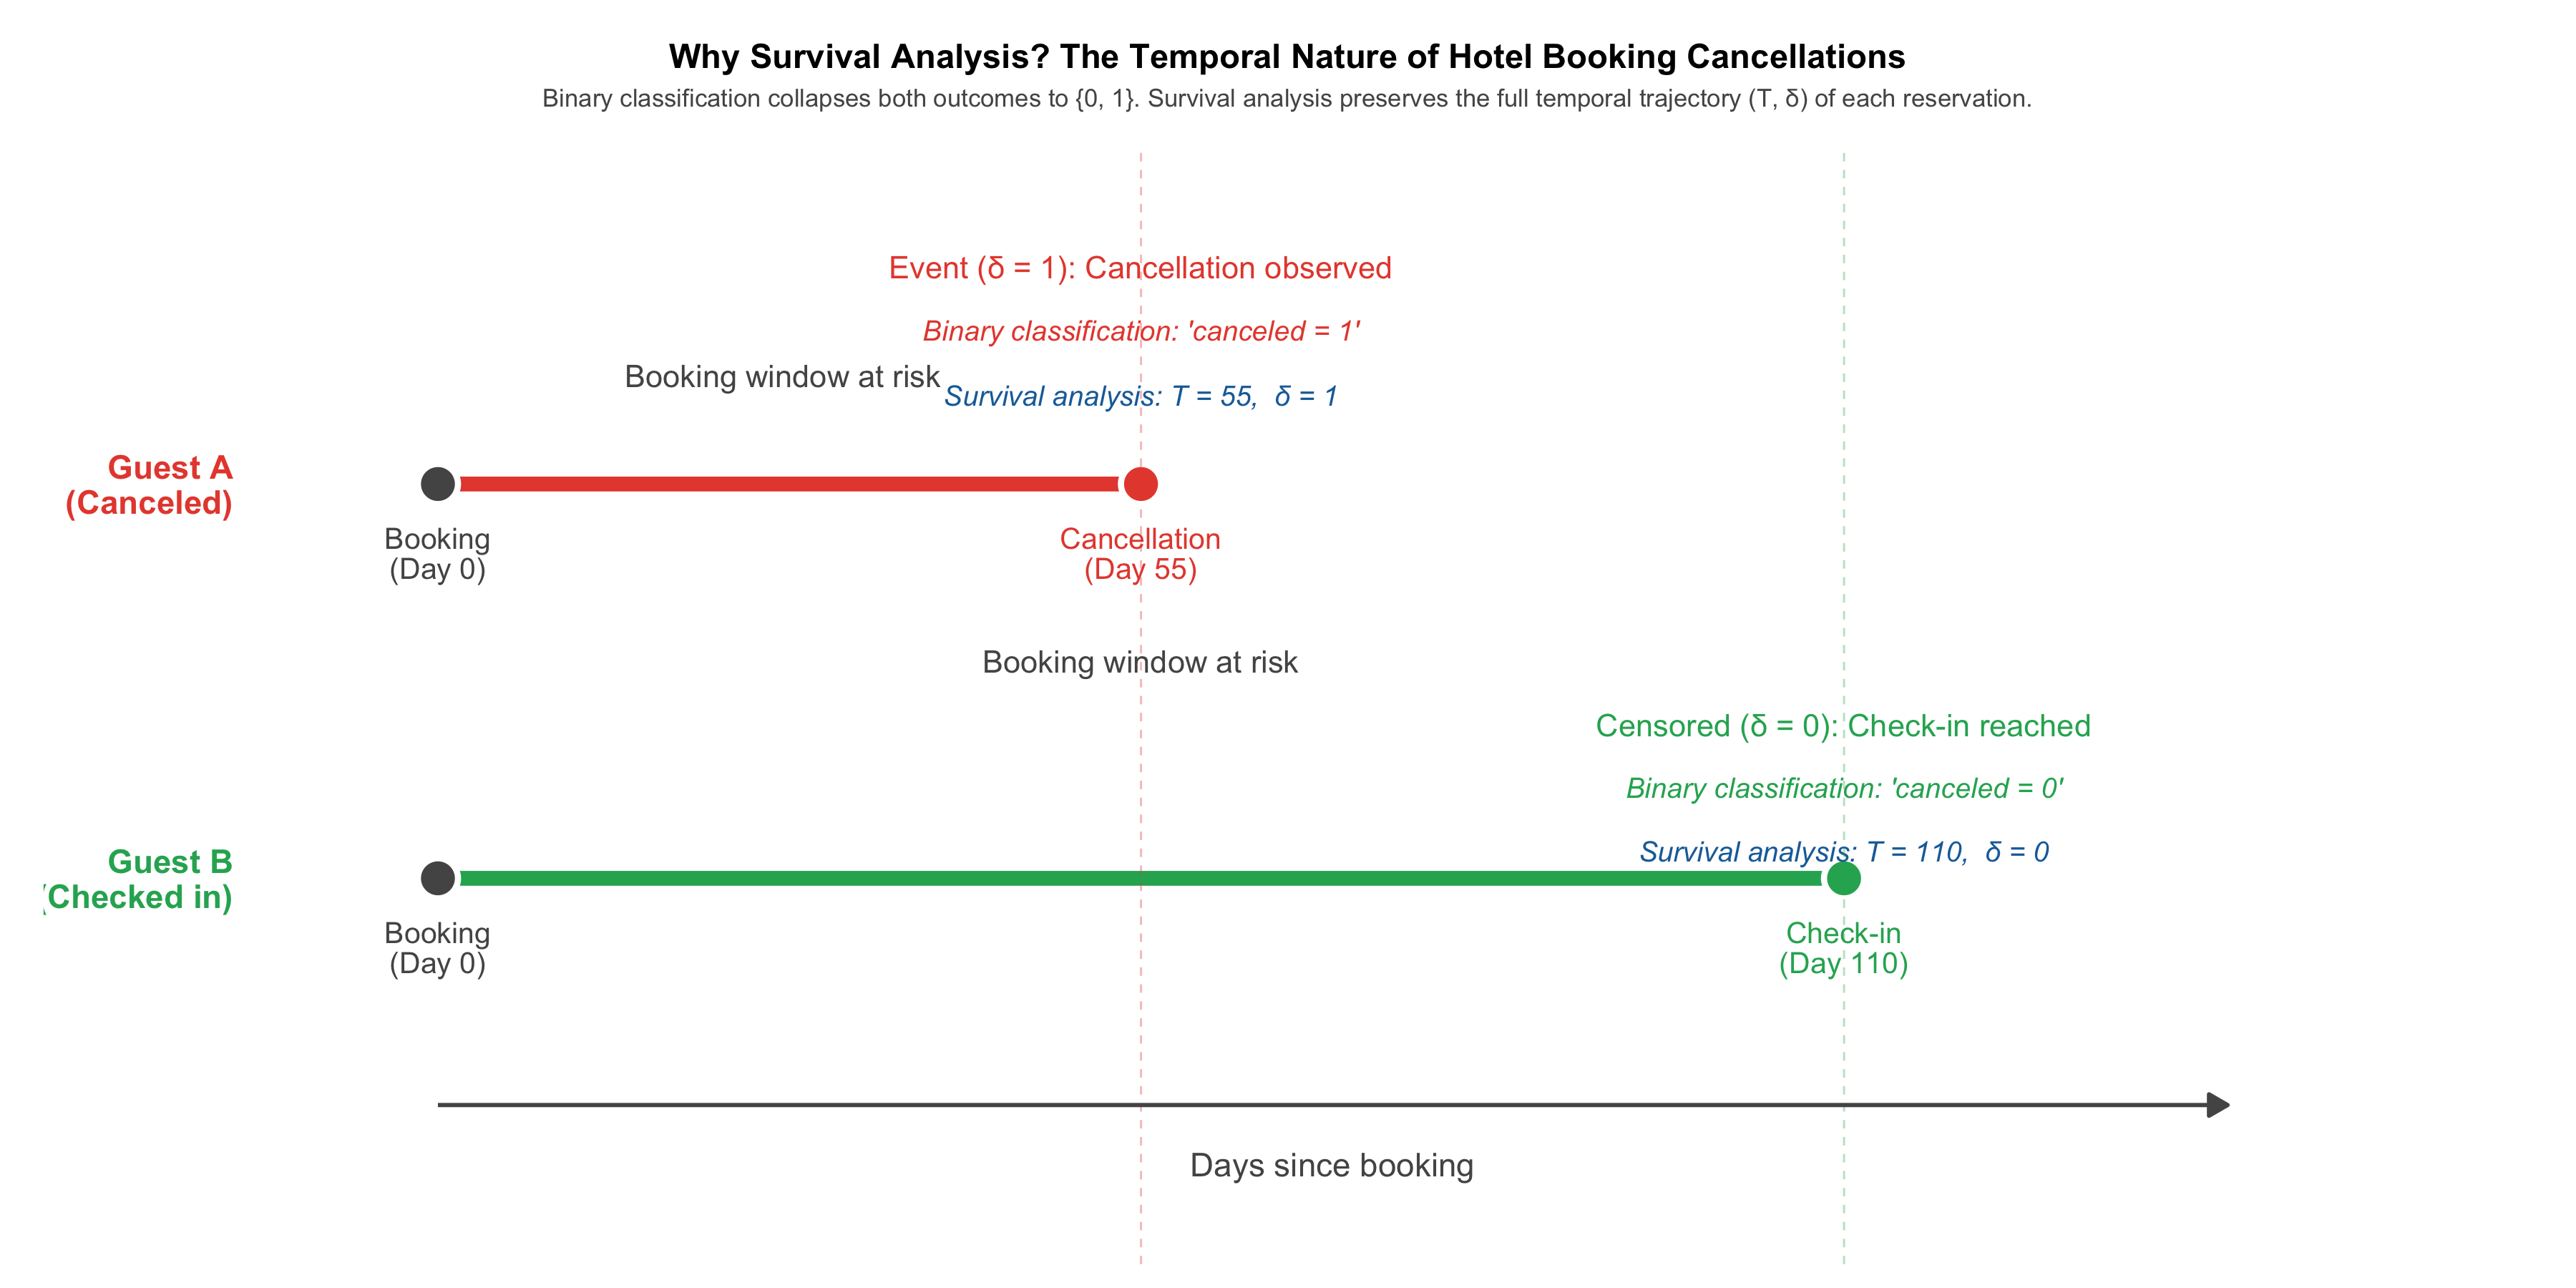
\includegraphics[width=0.95\textwidth]{fig_motivation.png}
\caption{Conceptual comparison of binary classification and survival analysis for hotel booking cancellations. Binary classification reduces both outcomes to a single binary label, discarding the temporal trajectory. Survival analysis preserves the full (Y, $\delta$) pair, enabling dynamic risk estimation over the booking window.}\label{fig:motivation}
\end{figure*}

\subsection{Time-to-Event Problem Formulation}

For a given $p$-dimensional feature vector $X \in \mathbb{R}^p$, the conditional survival function $S(t \mid X)$, which models the probability of a reservation remaining active beyond time $t$, is defined as:
\begin{equation}
S(t \mid X) = P(T > t \mid X)
\end{equation}
Correspondingly, the conditional hazard rate $\lambda(t \mid X)$, expressing the instantaneous rate of cancellation at time $t$ given survival up to that point, is formulated as:
\begin{align}
\lambda(t \mid X) &= \lim_{\Delta t \to 0} \frac{P(t \le T < t + \Delta t \mid T \ge t, X)}{\Delta t} \nonumber \\
         &= -\frac{d}{dt} \ln S(t \mid X)
\end{align}
By modeling $\hat{S}(t\mid X)$ directly using machine learning survival algorithms, we dynamically capture how cancellation risk changes over time.

Each observation in the training dataset takes the form $(X_i, Y_i, \delta_i)$, where $Y_i = \min(T_i, C_i)$ is the observed time (either the cancellation time $T_i$ or the censoring time $C_i$), and $\delta_i = \mathbf{1}(T_i \leq C_i)$ is the event indicator. Right-censoring arises when a booking has not been canceled by the time the dataset was compiled, the exact cancellation time is unknown, but it is known to exceed the observed duration. Survival models incorporate these censored observations through their likelihood contributions, avoiding the selection bias that contaminates binary classifiers when censored records are discarded or incorrectly labeled as non-events.

\subsection{Survival Model Families}

We benchmark ten survival algorithms spanning three methodological families. The \textbf{semi-parametric} family includes the classical Cox Proportional Hazards model, which assumes that the log-hazard ratio between any two covariate profiles is constant over time; Elastic Net Cox, which applies $\ell_1$/$\ell_2$ regularization to the Cox partial likelihood for variable selection in high-dimensional settings; and Gradient Boosted Cox, which iteratively fits Cox models to residuals via functional gradient descent, relaxing the global proportionality assumption. Component-wise Gradient Boosted Cox is a related approach that restricts each boosting step to a single predictor, producing sparse, interpretable models.

The \textbf{tree-based} family includes the Survival Tree, which maximizes log-rank test statistics at each split, and the Conditional Inference Tree, which replaces the greedy splitting criterion with conditional hypothesis tests, correcting for the selection bias toward high-cardinality variables that afflicts standard CART splits. The \textbf{ensemble} family comprises Random Survival Forests, which aggregate predictions from multiple survival trees grown on bootstrap samples with random feature subsets; Oblique Random Survival Forests, which replace axis-aligned splits with linear combinations of features, enabling curved decision boundaries that reduce survival function approximation error; and Conditional Survival Forests, which apply the CIT splitting strategy within an RSF framework to produce unbiased ensemble estimates. The Kaplan-Meier estimator serves as a non-parametric baseline that ignores covariates entirely.

The key distinction between standard RSF and Oblique RSF merits elaboration, as it directly explains the calibration differences observed in the results. In standard RSF, each internal node of each tree is split on a single feature at a single threshold, producing axis-aligned partition boundaries in the covariate space. This means that any non-linear survival surface that does not align with coordinate axes, such as an interaction between lead time and ADR that creates diagonal risk boundaries, requires many successive splits to approximate, introducing high variance in the estimated survival functions at leaf nodes. Oblique RSF addresses this by evaluating splits of the form $\sum_j w_j X_j \leq c$, where $w_j$ are feature weights optimized at each node. A single oblique split can capture a diagonal boundary that would require a deep subtree of axis-aligned splits to approximate, yielding smoother survival functions and better-calibrated probability estimates. The Conditional Survival Forest's advantage lies in a different dimension: by using permutation tests to determine split variable selection, it controls the family-wise error rate across variable comparisons, preventing the spurious selection of high-cardinality or correlated predictors that can distort both the splitting structure and the resulting survival estimates in datasets with mixed-type feature spaces such as those used in this study.

\subsection{Survival Partial Dependence Plots}

To capture the global marginal effect of a specific feature on the predicted survival probability across a continuous time horizon, we employ Survival Partial Dependence Plots (SurvPDP) proposed by \cite{langbein2025interpretable}, which generalizes classical Partial Dependence Plots originally formulated for tabular classification and regression by \cite{friedman2001greedy} to the time-to-event setting. Let $X$ represent the feature vector of size $p$, partitioned into a target feature of interest $X^S$ and the remaining features $X^C$ such that $X = (X^S, X^C)$. The survival function estimated by a machine learning survival model at time $t$ for a given feature configuration is denoted as $\hat{S}(t \mid X)$. The SurvPDP function for $X^S$ at time $t$ is defined by marginalizing over the joint distribution of $X^C$:
\begin{align}
\text{SurvPDP}(t, x^S) &= E_{X^C} \left[ \hat{S}(t \mid (x^S, X^C)) \right] \nonumber \\
            &\approx \frac{1}{N} \sum_{i=1}^N \hat{S}\left(t \mid (x^S, x_i^C)\right)
\end{align}
where $N$ is the number of observations in the dataset, and $x_i^C$ represents the values of the confounding features for the $i$-th instance. By plotting $\text{SurvPDP}(t, x^S)$ across a range of values for $x^S$ and continuous time steps $t$, we can visualize how the marginal survival curves and instantaneous cancellation risks evolve dynamically over the reservation lifecycle. Unlike SHAP values, which decompose a single scalar prediction, SurvPDPs produce a two-dimensional surface across feature values and time, offering a richer visualization of how a covariate's influence on the booking-to-cancellation trajectory changes as the check-in date approaches. This surface representation is particularly valuable for revenue management, as it allows analysts to identify the specific lead-time windows at which intervention is most effective for a given risk factor level.

\subsection{Survival Permutation Feature Importance}

To quantify the global impact of individual features on the survival model's overall predictive performance, we utilize Survival Permutation Feature Importance (SurvPFI) proposed by \cite{langbein2025interpretable}. This framework extends the foundational Permutation Feature Importance method originally introduced for tabular data by \cite{breiman2001random} into survival analysis by evaluating time-dependent loss functions. It measures the degradation in a model's predictive performance when the relationship between a target feature $X^j$ and the survival outcomes is broken via random shuffling.

Let $L(\hat{S}, D)$ represent a loss function, such as the Integrated Brier Score or one minus Harrell's concordance index, computed for the model $\hat{S}$ on the dataset $D = \{(X_i, Y_i, \delta_i)\}_{i=1}^N$. Let $D^{\pi, j}$ denote the perturbed dataset where the values of feature $X^j$ have been randomly permuted across observations while keeping all other features and target variables $(Y, \delta)$ intact. The permutation feature importance for feature $X^j$ is formulated as:
\begin{equation}
\text{SurvPFI}(X^j) = L(\hat{S}, D^{\pi, j}) - L(\hat{S}, D)
\end{equation}
Alternatively, it can be defined as the ratio $L(\hat{S}, D^{\pi, j}) / L(\hat{S}, D)$. Higher values of $\text{SurvPFI}(X^j)$ indicate that the model relies heavily on feature $X^j$ to predict time-to-event outcomes accurately. A key advantage of SurvPFI over standard PFI is that the loss function $L$ is evaluated at each time point $t$ along the survival horizon, yielding a curve rather than a scalar importance score. This time-resolved profile reveals whether a feature is uniformly important across the booking window, as is typical for structural attributes like deposit type, or whether its importance is concentrated in a specific temporal interval, as is characteristic of behavioral features like ADR whose influence compounds near check-in.

\begin{figure*}[htbp]
\centering
\resizebox{0.96\textwidth}{!}{
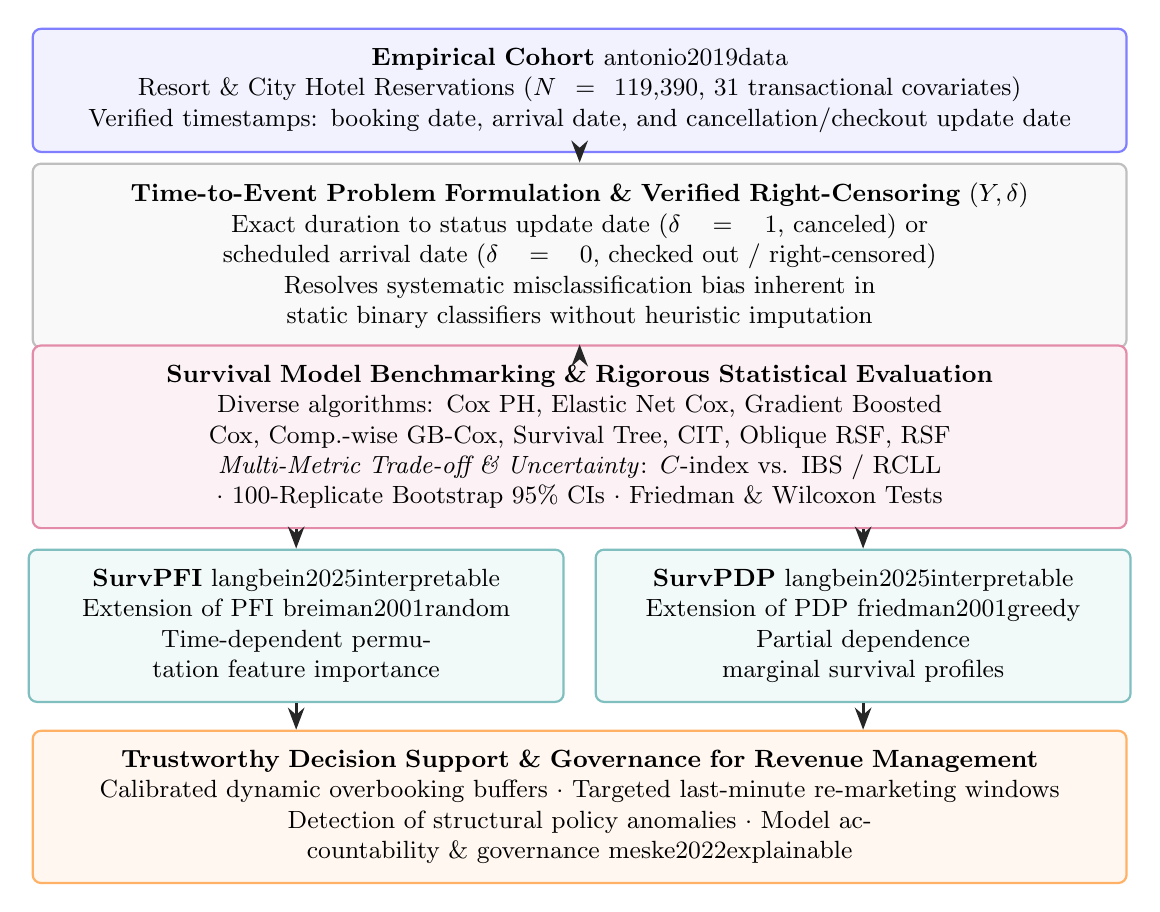
\begin{tikzpicture}[
  >=Stealth,
  every text node part/.style={align=center},
  basebox/.style={
    rectangle, 
    draw=black!75, 
    rounded corners=3pt, 
    font=\small, 
    inner sep=7pt,
    fill=white,
    line width=0.8pt
  },
  databox/.style={
    basebox, 
    fill=blue!5, 
    draw=blue!50, 
    text width=13.4cm
  },
  procbox/.style={
    basebox, 
    fill=gray!5, 
    draw=gray!50, 
    text width=13.4cm
  },
  modelbox/.style={
    basebox, 
    fill=purple!5, 
    draw=purple!45, 
    text width=13.4cm
  },
  xaibox/.style={
    basebox, 
    fill=teal!5, 
    draw=teal!50, 
    text width=6.3cm
  },
  outbox/.style={
    basebox, 
    fill=orange!6, 
    draw=orange!60, 
    text width=13.4cm
  },
  arrowline/.style={
    ->, 
    draw=black!85, 
    line width=1.1pt
  }
]

% 1. Dataset
\node[databox] (d1) at (0, 0) {\textbf{Empirical Cohort} \citep{antonio2019data}\\ Resort \& City Hotel Reservations ($N=119{,}390$, 31 transactional covariates)\\ Verified timestamps: booking date, arrival date, and cancellation/checkout update date};

% 2. TTE Formulation
\node[procbox] (tte) at (0, -2.1) {
  \textbf{Time-to-Event Problem Formulation \& Verified Right-Censoring $(Y, \delta)$}\\
  Exact duration to status update date ($\delta=1$, canceled) or scheduled arrival date ($\delta=0$, checked out / right-censored)\\
  Resolves systematic misclassification bias inherent in static binary classifiers without heuristic imputation
};

% 3. Benchmarking & Statistical Evaluation
\node[modelbox] (models) at (0, -4.4) {
  \textbf{Survival Model Benchmarking \& Rigorous Statistical Evaluation}\\
  Diverse algorithms: Cox PH, Elastic Net Cox, Gradient Boosted Cox, Comp.-wise GB-Cox, Survival Tree, CIT, Oblique RSF, RSF\\
  \textit{Multi-Metric Trade-off \& Uncertainty}: $C$-index vs. IBS / RCLL $\cdot$ 100-Replicate Bootstrap 95\% CIs $\cdot$ Friedman \& Wilcoxon Tests
};

% 4. XAI Split
\coordinate (m_mid) at (models.south);
\node[xaibox] (pfi) at (-3.6, -6.8) {
  \textbf{SurvPFI} \citep{langbein2025interpretable}\\
  Extension of PFI \citep{breiman2001random}\\
  Time-dependent permutation feature importance
};

\node[xaibox] (pdp) at (3.6, -6.8) {
  \textbf{SurvPDP} \citep{langbein2025interpretable}\\
  Extension of PDP \citep{friedman2001greedy}\\
  Partial dependence marginal survival profiles
};

% 5. Decision Support
\coordinate (xai_mid) at ($(pfi.south)!0.5!(pdp.south)$);
\node[outbox] (out) at (0, -9.1) {
  \textbf{Trustworthy Decision Support \& Governance for Revenue Management}\\
  Calibrated dynamic overbooking buffers $\cdot$ Targeted last-minute re-marketing windows\\
  Detection of structural policy anomalies $\cdot$ Model accountability \& governance \citep{meske2022explainable}
};

% Connectors
\draw[arrowline] (d1.south) -- (tte.north);
\draw[arrowline] (tte.south) -- (models.north);
\draw[arrowline] (models.south -| pfi.north) -- (pfi.north);
\draw[arrowline] (models.south -| pdp.north) -- (pdp.north);
\draw[arrowline] (pfi.south) -- (pfi.south |- out.north);
\draw[arrowline] (pdp.south) -- (pdp.south |- out.north);

\end{tikzpicture}
}
\caption{Overview of the proposed explainable time-to-event modeling framework. The pipeline proceeds from verified reservation transaction data through survival duration construction, multi-algorithm benchmarking with statistical uncertainty estimation, and time-dependent XAI analysis, culminating in trustworthy, actionable insights for RM.}\label{fig:framework}
\end{figure*}

\section{Experimental Design}
%%%%%%%%%%%%%%%%%%%%%%%%%%%%%%%%%%%%%%%%%%%%%%%%%%%
\label{sec:experimental_design}

This section describes the empirical datasets used to validate the proposed framework, details the survival duration construction procedure for each dataset, and outlines the data preprocessing steps, model training protocol, and evaluation pipeline. The full experimental workflow is depicted in Figure~\ref{fig:pipeline}.

\subsection{Empirical Dataset and Verified Time-to-Event Construction}
\label{sec:dataset}

To evaluate the proposed explainable time-to-event framework and ensure the empirical integrity of temporal cancellation forecasting, we analyze the benchmark Hotel Booking Demand cohort originally collected by \cite{antonio2019data}. Unlike secondary booking archives that lack event tracking, this dataset comprises $119{,}390$ individual reservation transactions recorded from a Resort Hotel and a City Hotel in Portugal, spanning from July 2015 to August 2017. The feature space contains $31$ covariates encompassing reservation characteristics such as lead time, arrival date, length of stay, and assigned room type, customer historical interactions such as prior cancellations, booking modifications, and repeat guest status, and transactional parameters including average daily rate, deposit policy, market segment, and distribution channel.

A foundational methodological requirement for survival analysis is the exact measurement of duration ($T$) and censoring status ($\delta$). In this study, the survival duration is constructed strictly from verified operational timestamps:
\begin{enumerate}
  \item \textbf{Canceled Reservations ($\delta = 1$)}: For bookings where the customer or intermediary terminated the contract, the duration $T_i$ represents the exact number of days elapsed between the reservation creation timestamp ($\text{Arrival Date}_i - \text{Lead Time}_i$) and the formal status update timestamp recorded in the hotel property management system.
  \item \textbf{Active / Checked-Out Reservations ($\delta = 0$)}: For reservations that were honored, the duration $T_i$ represents the complete booking horizon elapsed between the reservation creation timestamp and the scheduled arrival date, at which point the observation is right-censored.
\end{enumerate}
By computing exact survival times from verified operational records, this formulation completely eliminates the necessity for artificial midpoint imputation or heuristic cancellation proxies, ensuring that model predictions reflect true operational attrition patterns.

A detailed statistical characterization of all features in the empirical cohort, including measurement scales and domain distributions, is structured in Table~\ref{tab:dataset_comparison}.

\begin{table*}[htbp]
\centering
\small
\caption{Comprehensive feature dictionary, measurement scales, and descriptive distributions of the empirical hotel booking cohort}\label{tab:dataset_comparison}
\begin{tabular*}{\textwidth}{@{\extracolsep{\fill}} p{0.24\textwidth} p{0.36\textwidth} p{0.34\textwidth}}
\toprule
Variable & Domain or Levels & Description \\
\midrule
\textit{Continuous and Temporal Covariates} & & \\
\midrule
Lead Time & $[0, 737]$ days & Days elapsed between booking creation and check-in \\
Average Daily Rate & $[-6.38, 5400.00]$ EUR & Average rental revenue per occupied room per day \\
Stays in Weekend Nights & $[0, 19]$ nights & Number of weekend nights booked on Saturday or Sunday \\
Stays in Week Nights & $[0, 50]$ nights & Number of week nights booked from Monday through Friday \\
Days in Waiting List & $[0, 391]$ days & Number of days the booking was in the waiting list \\
\midrule
\textit{Demographics and Behavioral Counts} & & \\
\midrule
Number of Adults & $[0, 55]$ & Number of adults included in the reservation \\
Number of Children & $[0, 10]$ & Number of children accompanying the booking \\
Number of Babies & $[0, 10]$ & Number of infants accompanying the booking \\
Previous Cancellations & $[0, 26]$ & Number of previous bookings canceled by the customer \\
Previous Stays Not Canceled & $[0, 72]$ & Number of previous successful stays by the customer \\
Booking Changes & $[0, 21]$ & Modifications made to the reservation before check-in \\
Total Special Requests & $[0, 5]$ & Special customer requests such as high floor or twin bed \\
Required Parking Spaces & $[0, 8]$ & Number of parking spaces requested by the customer \\
\midrule
\textit{Categorical and Policy Covariates} & & \\
\midrule
Hotel Type & \{\text{City Hotel}, \text{Resort Hotel}\} & Type of lodging facility \\
Deposit Type & \{\text{No Deposit}, \text{Non-Refund}, \text{Refundable}\} & Financial guarantee required to confirm the booking \\
Market Segment & \{\text{Direct}, \text{Corporate}, \text{Online TA}, \text{Offline TA/TO}, \text{Groups}, \text{Aviation}\} & Market designation segment \\
Distribution Channel & \{\text{Direct}, \text{Corporate}, \text{TA/TO}, \text{GDS}\} & Intermediary booking channel \\
Customer Type & \{\text{Transient}, \text{Contract}, \text{Transient-Party}, \text{Group}\} & Customer category classification \\
Reserved Room Type & \{\text{A}, \text{B}, \text{C}, \text{D}, \text{E}, \text{F}, \text{G}, \text{H}, \text{L}\} & Code of room type reserved by guest \\
Assigned Room Type & \{\text{A}, \text{B}, \text{C}, \text{D}, \text{E}, \text{F}, \text{G}, \text{H}, \text{I}, \text{K}, \text{P}\} & Code for room type actually assigned at check-in \\
Meal Plan & \{\text{BB}, \text{FB}, \text{HB}, \text{SC}, \text{Undefined}\} & Type of meal booked such as Bed and Breakfast \\
\midrule
\textit{Survival Response Pair} & & \\
\midrule
Survival Time $T$ & $[0, 737]$ days & Exact elapsed duration to event or right-censoring \\
Event Status $\delta$ & $\delta=1$ for Canceled [37.04\%], $\delta=0$ for Checked-out [62.96\%] & Right-censoring indicator \\
\bottomrule
\end{tabular*}
\end{table*}


\subsection{Data Preprocessing and Quality Control}

Prior to survival modeling, the empirical cohort underwent a systematic cleaning and quality assurance protocol following established hospitality benchmarking practices \citep{antonio2019data}. First, observations with physically implausible entries, specifically, reservations recording zero total guests with no registered adults, children, or babies, negative ADR values arising from accounting adjustments or reversals, and exact duplicate transaction records, were removed. Categorical variables, including hotel type, deposit type, market segment, distribution channel, customer type, room types, and meal plan, were encoded as nominal factors. Ordinal count variables, including prior cancellations, booking modifications, and special requests, were preserved as integers.

Missing values were negligible under 0.5\% across all fields and handled via median imputation for continuous attributes and mode imputation for categorical predictors. No synthetic oversampling or undersampling was applied to artificially manipulate the event distribution; the empirical cancellation rate of 37.04\% reflects natural hotel demand conditions, and survival analysis likelihood frameworks inherently accommodate asymmetric censoring proportions without distortion. Feature scaling was omitted, as non-parametric tree-based ensemble models are strictly invariant to monotonic predictor transformations.

The empirical censoring rate, representing reservations that reached successful check-in without cancellation ($\delta = 0$), is 62.96\%. In conventional binary classification pipelines, these active reservations create a fundamental dilemma: either they are discarded, causing substantial sample selection bias, or they are naively labeled as non-cancellations, introducing severe right-censoring bias. Survival analysis eliminates this vulnerability by properly factoring the censored duration into the partial likelihood and inverse probability of censoring weighting evaluation metrics.

\subsection{Model Training, Resampling, and Statistical Validation Pipeline}
\label{sec:experiments}

To rigorously evaluate predictive generalizability and quantify estimation uncertainty, we implemented a rigorous nested evaluation protocol. The empirical dataset was first partitioned into an 80\% training partition ($N_{\text{train}} = 95{,}512$) and an independent 20\% held-out test partition ($N_{\text{test}} = 23{,}878$) using stratified random sampling to preserve the exact empirical censoring ratio ($\delta = 37.04\%$ canceled) across splits. The entire experimental workflow was orchestrated using the \texttt{mlr3proba} survival analysis ecosystem in R.

Within the training partition, internal model stability was monitored via stratified 10-fold cross-validation. Hyperparameter search configurations and baseline model fits were performed strictly on training data. Following model fitting, out-of-sample predictive performance was evaluated on the untouched 20\% held-out test partition across four complementary metrics:
\begin{enumerate}
  \item \textbf{Concordance Index ($C$-index)}: Evaluates the discriminative ordering capacity of predicted survival risks, where higher values indicate superior discrimination and 0.5 denotes random guessing.
  \item \textbf{Integrated Brier Score (IBS)}: Measures probability calibration error across continuous time using inverse probability of censoring weighting, where lower values indicate superior calibration.
  \item \textbf{Right-Censored Log-Likelihood (RCLL)}: Assesses the probabilistic likelihood of true event times under the predicted distribution, where lower values indicate superior probabilistic fit.
\end{enumerate}

To address the absence of variance estimates and statistical hypothesis testing in prior studies, we conducted $B = 100$ independent non-parametric bootstrap resamples on the held-out test partition. For each bootstrap iteration $b \in \{1, \dots, 100\}$, the test set was sampled with replacement, and out-of-sample metrics were computed across all models simultaneously. This enables the direct reporting of:
\begin{itemize}
  \item \textbf{Empirical standard deviations ($\text{SD}$)} and \textbf{95\% non-parametric bootstrap confidence intervals}.
  \item \textbf{Omnibus hypothesis testing}: A non-parametric Friedman test across bootstrap replicates to determine whether performance differentials across algorithms are statistically significant.
  \item \textbf{Post-hoc pairwise comparisons}: Paired Wilcoxon signed-rank tests with Bonferroni correction comparing all benchmarked algorithms against the top-performing model.
\end{itemize}

Finally, to address whether survival models deliver genuine probability calibration rather than mere ranking accuracy, we generated empirical calibration curves across multiple forward-looking horizons ($t \in \{30, 60, 90, 180\}$ days). Predicted survival probabilities were partitioned into deciles and benchmarked against non-parametric Kaplan-Meier survival estimates computed within each bin.

Crucially, all model explanations, both SurvPFI and SurvPDP, were extracted strictly on the untouched 20\% held-out test set to prevent training-data memorization and reflect true operational conditions. The full experimental design is illustrated in Figure~\ref{fig:pipeline}.

\begin{figure*}[htbp]
\centering
\resizebox{0.92\textwidth}{!}{
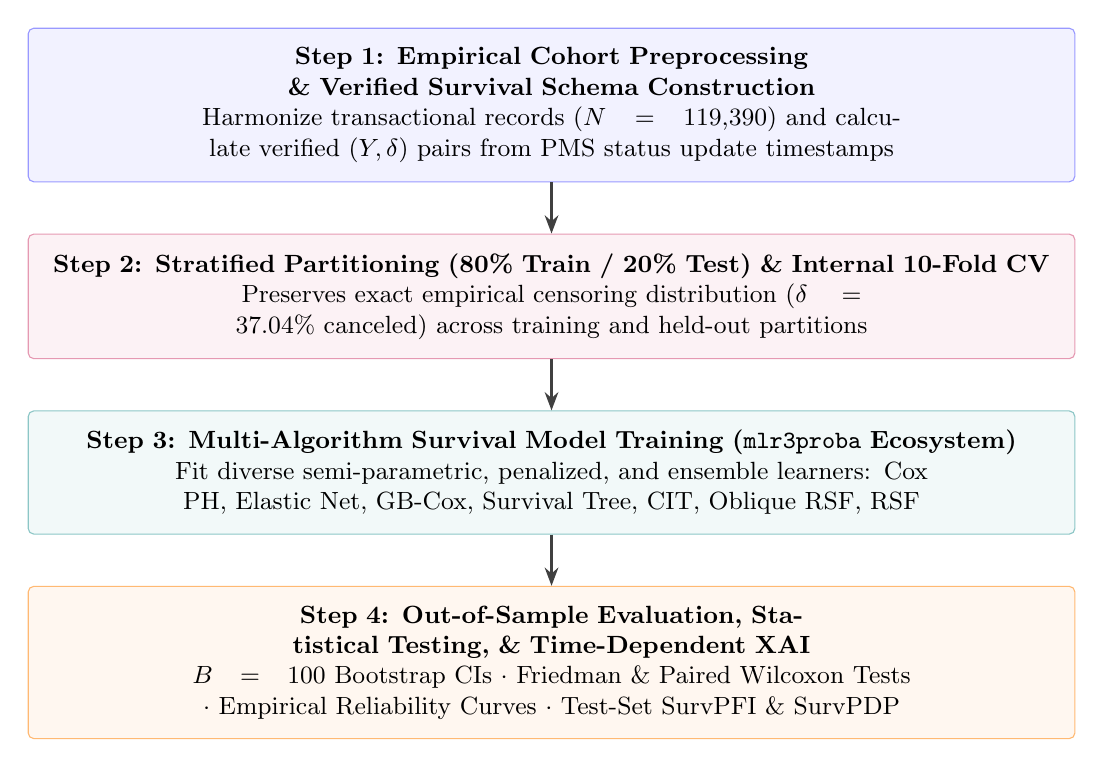
\begin{tikzpicture}[
  >=Stealth,
  node distance=0.65cm,
  every text node part/.style={align=center},
  pipebox/.style={
    rectangle, 
    draw=black!70, 
    rounded corners=2pt, 
    font=\small, 
    inner sep=7pt,
    fill=white,
    text width=12.8cm
  },
  stepbox/.style={
    pipebox,
    fill=blue!5,
    draw=blue!40
  },
  splitbox/.style={
    pipebox,
    fill=purple!5,
    draw=purple!40
  },
  trainbox/.style={
    pipebox,
    fill=teal!5,
    draw=teal!45
  },
  evalbox/.style={
    pipebox,
    fill=orange!6,
    draw=orange!55
  },
  arrowline/.style={
    ->, 
    draw=black!75, 
    line width=0.8pt
  }
]

\node[stepbox] (p1) {
  \textbf{Step 1: Empirical Cohort Preprocessing \& Verified Survival Schema Construction}\\
  Harmonize transactional records ($N=119{,}390$) and calculate verified $(Y, \delta)$ pairs from PMS status update timestamps
};

\node[splitbox, below=0.65cm of p1] (p2) {
  \textbf{Step 2: Stratified Partitioning (80\% Train / 20\% Test) \& Internal 10-Fold CV}\\
  Preserves exact empirical censoring distribution ($\delta = 37.04\%$ canceled) across training and held-out partitions
};

\node[trainbox, below=0.65cm of p2] (p3) {
  \textbf{Step 3: Multi-Algorithm Survival Model Training (\texttt{mlr3proba} Ecosystem)}\\
  Fit diverse semi-parametric, penalized, and ensemble learners: Cox PH, Elastic Net, GB-Cox, Survival Tree, CIT, Oblique RSF, RSF
};

\node[evalbox, below=0.65cm of p3] (p4) {
  \textbf{Step 4: Out-of-Sample Evaluation, Statistical Testing, \& Time-Dependent XAI}\\
  $B = 100$ Bootstrap CIs $\cdot$ Friedman \& Paired Wilcoxon Tests $\cdot$ Empirical Reliability Curves $\cdot$ Test-Set SurvPFI \& SurvPDP
};

\draw[arrowline] (p1) -- (p2);
\draw[arrowline] (p2) -- (p3);
\draw[arrowline] (p3) -- (p4);

\end{tikzpicture}
}
\caption{Experimental pipeline for model training, statistical uncertainty estimation, and out-of-sample explanation on the empirical hotel booking cohort.}\label{fig:pipeline}
\end{figure*}

\section{Results}
\label{sec:results}

This section presents the empirical findings of the study across three complementary dimensions. First, we compare the out-of-sample predictive performance of the benchmarked survival models on the independent held-out test partition ($N_{\text{test}} = 23{,}878$), incorporating statistical uncertainty estimation and hypothesis testing. Second, we evaluate genuine probability calibration across forward-looking horizons via reliability diagrams. Third, we deploy continuous time-dependent explainable AI tools, specifically SurvPFI and SurvPDP, to audit the model's internal risk logic.

\subsection{Model Performance Comparison and Statistical Inference}
\label{sec:performance_comparison}

Table~\ref{tab:performance_comparison} presents the out-of-sample benchmark results for all survival analysis algorithms evaluated on the independent $20\%$ held-out test partition ($N_{\text{test}} = 23{,}878$). To provide rigorous statistical validation, we report point estimates, empirical standard deviations, and $95\%$ non-parametric bootstrap confidence intervals computed across $B = 100$ resamples. Furthermore, statistical significance was evaluated using a Friedman test across bootstrap replicates, followed by post-hoc paired Wilcoxon signed-rank tests with Bonferroni correction comparing all models against the top-ranking algorithm.

\begin{table*}[htbp]
\centering
\small
\caption{Out-of-sample predictive performance, statistical uncertainty across bootstrap iterations, and calibration loss on the held-out test partition}\label{tab:performance_comparison}
\begin{tabular*}{\textwidth}{@{\extracolsep{\fill}} lccccc}
\toprule
Model & $C$-index (Point) & $C$-index ($\text{Mean} \pm \text{SD}$) & 95\% Bootstrap CI & IBS $\downarrow$ & RCLL $\downarrow$ \\
\midrule
Standard RSF & \textbf{0.8049} & $0.8090 \pm 0.0025$ & $[0.8039, 0.8135]$ & 0.1331 & 1.7387 \\
Oblique RSF & 0.7855 & $0.7879 \pm 0.0028^*$ & $[0.7819, 0.7923]$ & \textbf{0.0844} & \textbf{1.5865} \\
Cox PH & 0.7776 & $0.7758 \pm 0.0029^*$ & $[0.7702, 0.7811]$ & 0.0842 & 2.0268 \\
Gradient Boosted Cox & 0.7654 & $0.7640 \pm 0.0029^*$ & $[0.7587, 0.7696]$ & 0.0957 & 2.0601 \\
Elastic Net Cox & 0.7550 & $0.7511 \pm 0.0033^*$ & $[0.7450, 0.7574]$ & 0.0898 & 2.0723 \\
Survival Tree & 0.7329 & $0.7342 \pm 0.0030^*$ & $[0.7287, 0.7396]$ & -- & -- \\
Component-wise GB-Cox & 0.7214 & $0.7149 \pm 0.0035^*$ & $[0.7082, 0.7211]$ & 0.1045 & 2.1143 \\
Kaplan-Meier Baseline & 0.5000 & $0.5000 \pm 0.0000^*$ & $[0.5000, 0.5000]$ & 0.1487 & 2.2295 \\
\bottomrule
\end{tabular*}
\footnotetext{Notes: $C$-index: Harrell's Concordance Index; IBS: Integrated Brier Score; RCLL: Right-Censored Log-Loss. ($*$) indicates that the discriminative performance difference relative to top-performing Standard RSF is statistically significant at $p < 10^{-15}$ based on paired Wilcoxon signed-rank tests across bootstrap iterations. The omnibus Friedman test across all models confirms significant overall divergence ($\chi^2 = 789.2$, $p < 10^{-15}$). A dash indicates non-parametric single-tree models that do not natively produce continuous predictive distribution functions.}
\end{table*}

\subsubsection{Discriminative Concordance and Statistical Significance}
The empirical benchmarking demonstrates substantial discriminative capabilities across all machine learning architectures relative to the non-informative Kaplan-Meier baseline ($C$-index = $0.5000$). Ensemble tree architectures achieve the strongest risk ranking: Standard RSF attains the highest test $C$-index ($0.8049 \pm 0.0025$, $95\%$ CI: $[0.8039, 0.8135]$), closely followed by Oblique RSF ($0.7855 \pm 0.0028$) and Cox PH ($0.7776 \pm 0.0029$). The narrow width of the $95\%$ bootstrap confidence intervals across all learners (less than $\pm 0.006$) demonstrates strong statistical stability and confirms that performance gaps do not stem from test-set sampling artifacts.

The omnibus non-parametric Friedman test indicates that predictive differences among models are highly statistically significant ($\chi^2 = 789.2$, $p < 10^{-15}$). Pairwise post-hoc Wilcoxon signed-rank tests with Bonferroni correction confirm that Standard RSF significantly outperforms all competing learners in pure discriminative ranking ($p < 10^{-15}$ across all pairwise comparisons).

\subsubsection{The Concordance versus Probability Calibration Trade-off}
Crucially, evaluating models solely on discriminative ranking ($C$-index) masks a fundamental trade-off that is vital for hotel revenue management: \textit{rank concordance versus probability calibration}. While Standard RSF achieves top-tier concordance, it exhibits poor probability calibration, yielding an Integrated Brier Score of $0.1331$ and an RCLL of $1.7387$. In contrast, Oblique RSF delivers superior probability calibration, achieving an IBS of $0.0844$ and the lowest RCLL ($1.5865$) across the entire benchmark cohort, while remaining highly competitive in concordance ($C$-index = $0.7855$).

\begin{figure*}[htbp]
\centering
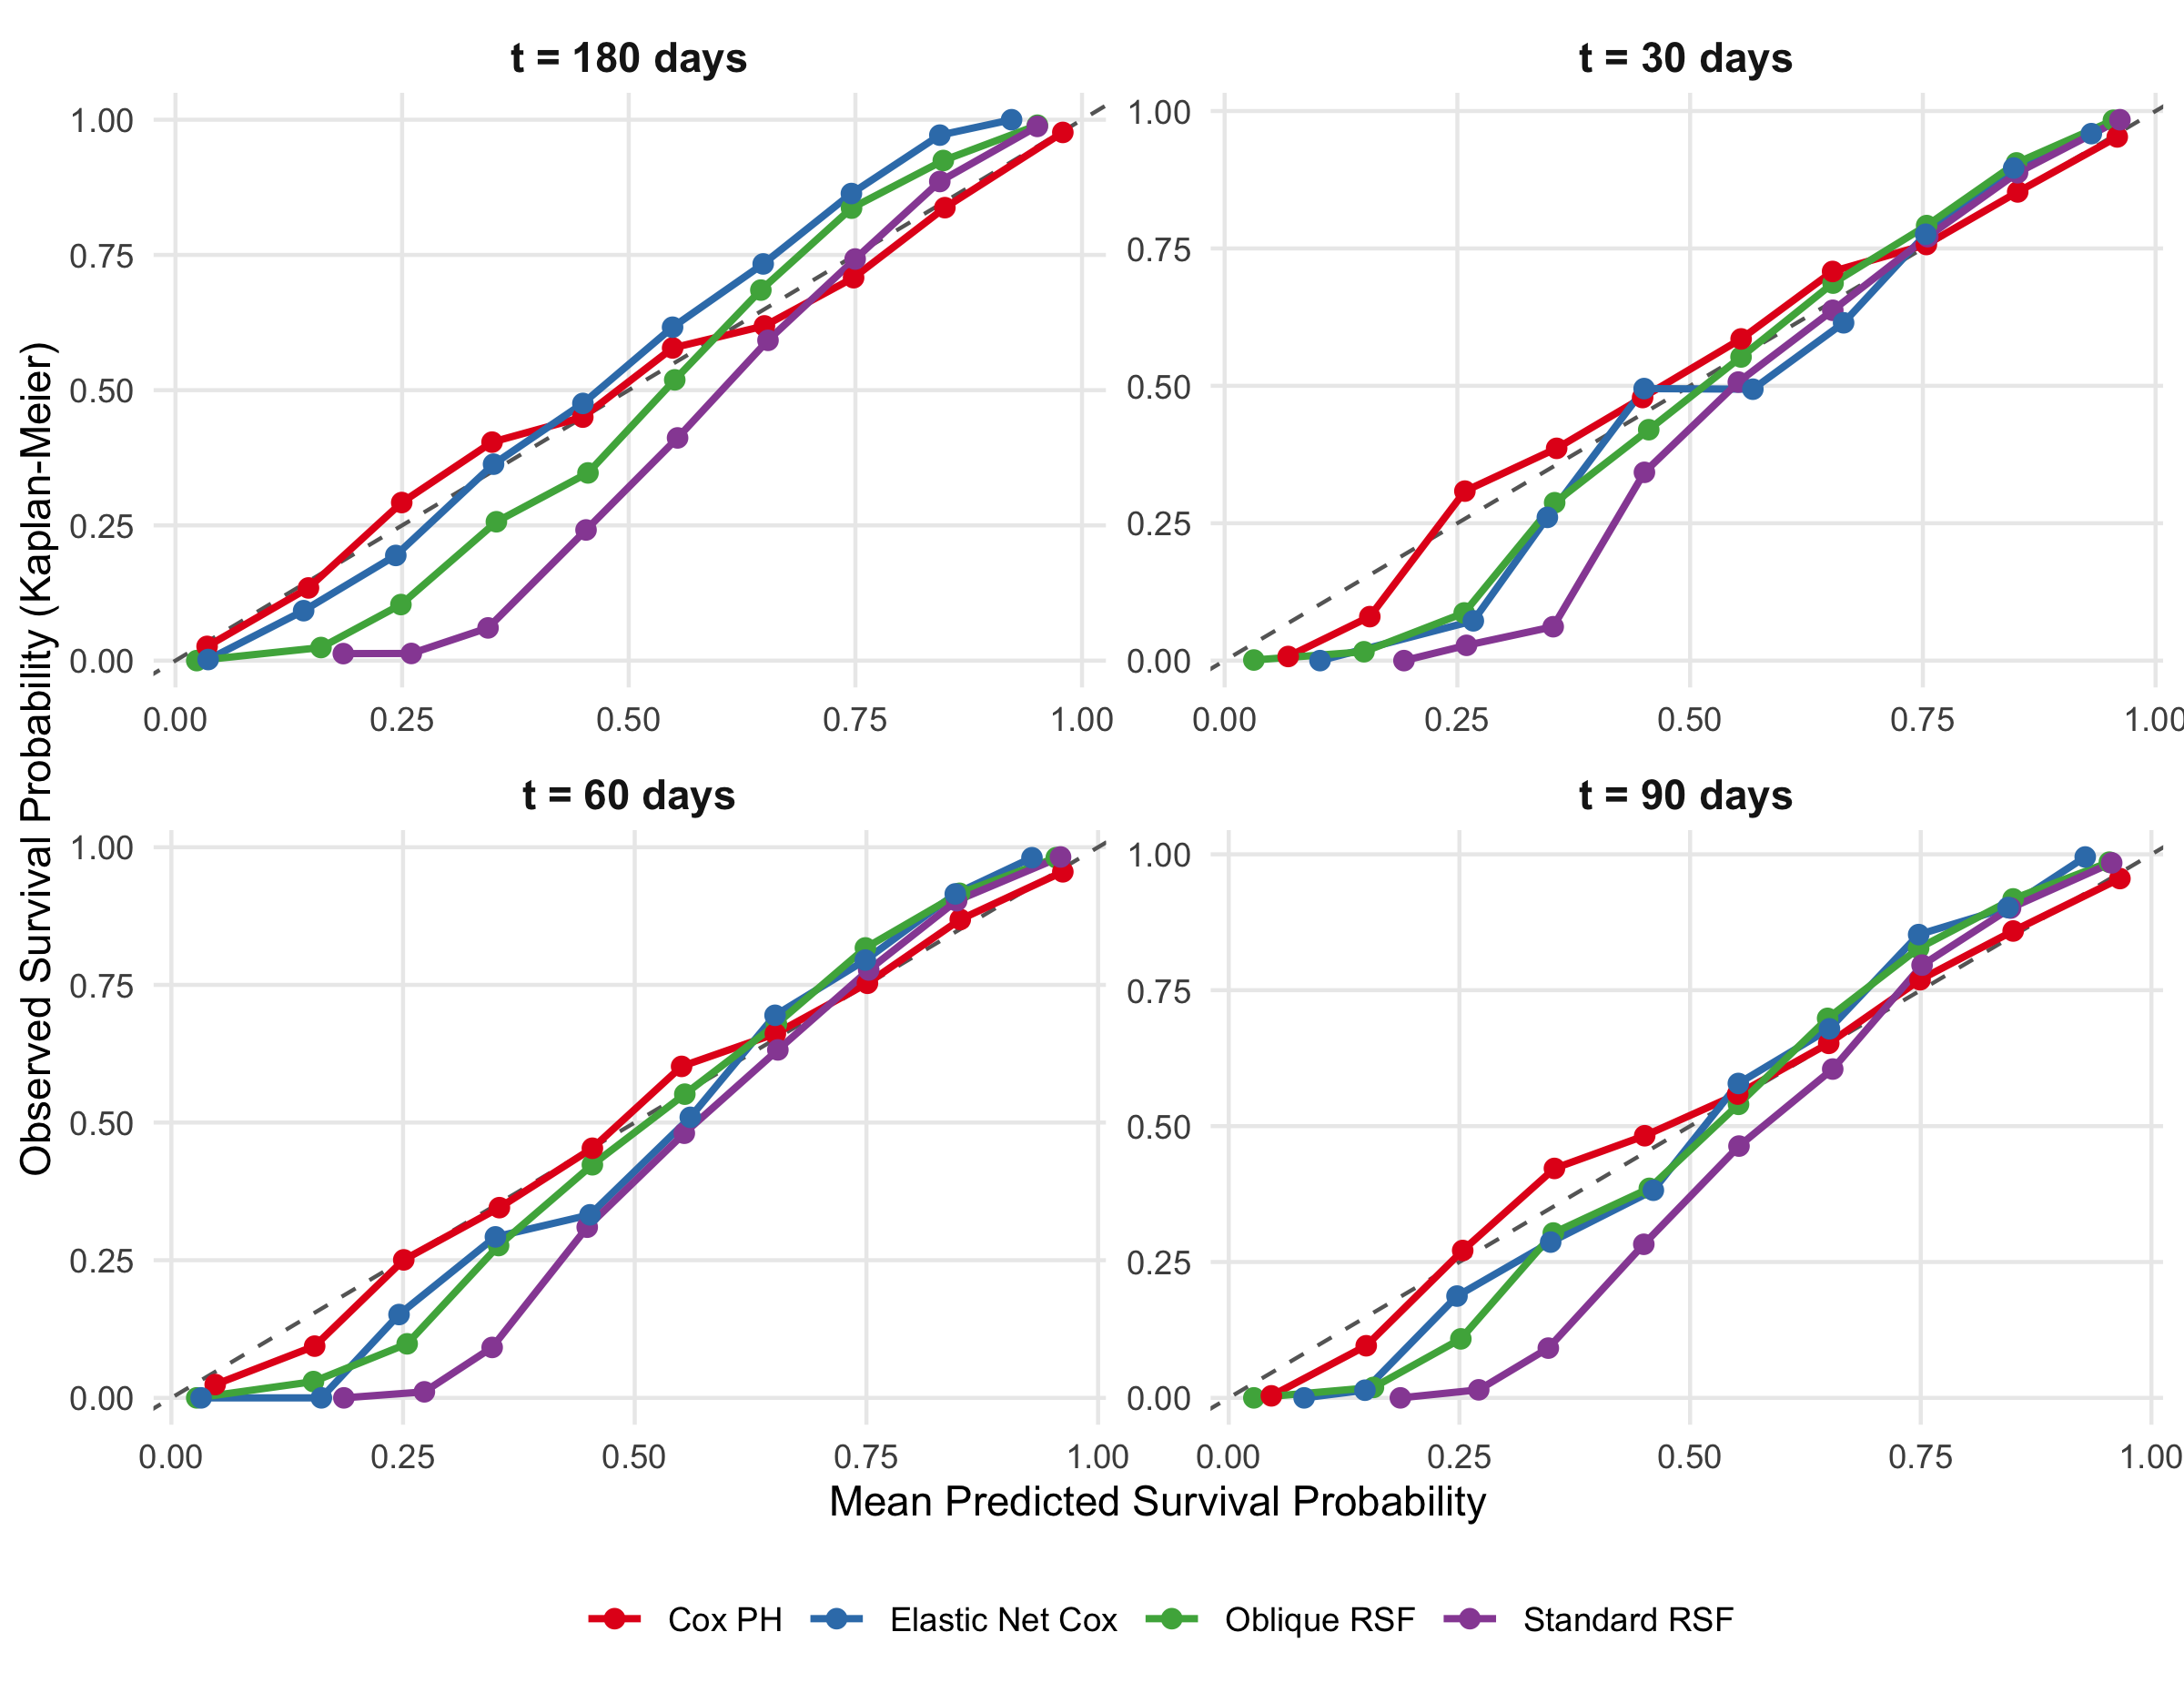
\includegraphics[width=0.92\textwidth]{fig_calibration_curves.png}
\caption{Empirical probability calibration curves across four operational horizons. Mean predicted survival probabilities within decile bins are evaluated against non-parametric Kaplan-Meier observed survival rates on the independent held-out test partition. The diagonal dashed line denotes perfect probability calibration.}\label{fig:calibration}
\end{figure*}

To evaluate genuine probability calibration beyond summary scalar metrics, Figure~\ref{fig:calibration} presents empirical calibration curves across four operational planning horizons ($t = 30, 60, 90,$ and $180$ days). For each horizon, predicted survival probabilities are binned into deciles and plotted against the observed Kaplan-Meier event rate within each bin. The visual inspection rigorously substantiates the quantitative IBS results:
\begin{enumerate}
  \item \textbf{Oblique RSF and Cox PH} track the ideal 45-degree diagonal line with high fidelity across all four operational horizons. Their predicted probabilities accurately reflect actual empirical non-cancellation proportions across the full spectrum from high-risk to low-risk reservations.
  \item \textbf{Standard RSF}, despite its superior ranking concordance, deviates substantially from the diagonal line across all time horizons. It systematically over-predicts survival for moderate-risk bookings and compresses probability mass toward the center.
\end{enumerate}

For operational revenue management systems, this calibration advantage is decisive: setting dynamic overbooking quotas, allocating distressed room inventory, and establishing optimal refund penalties require \textit{accurate expected values and calibrated probabilities}, rather than mere ordinal rankings.

\subsection{Model Explanations via Time-Dependent XAI}
\label{sec:explanations}

To transcend static black-box predictions and decode the temporal risk dynamics of booking cancellations, we deploy the time-dependent Survival Permutation Feature Importance and Partial Dependence Survival Profiles frameworks \citep{langbein2025interpretable}. SurvPFI quantifies the marginal degradation in the Brier Score when a specific feature is permuted across the continuous survival time horizon. Crucially, to reflect authentic operational conditions and guard against data leakage, all model explanations are computed strictly on the completely untouched $20\%$ held-out test partition. We extract these explanations from the best-calibrated model, Oblique RSF.

Figure~\ref{fig:survpfi_ds1} illustrates the time-dependent SurvPFI curves across the continuous reservation window. The temporal trajectory reveals a striking non-linear escalation in the predictive reliance of three primary structural variables: \texttt{lead\_time}, \texttt{market\_segment}, and \texttt{deposit\_type}. While the influence of most static demographic attributes remains comparatively modest, the predictive impact of \texttt{lead\_time} compounds significantly as the booking horizon matures. Furthermore, \texttt{deposit\_type} exhibits a consistently elevated predictive influence from the moment the reservation is created, confirming its role as an essential baseline risk determinant.

\begin{figure*}[htbp]
\centering
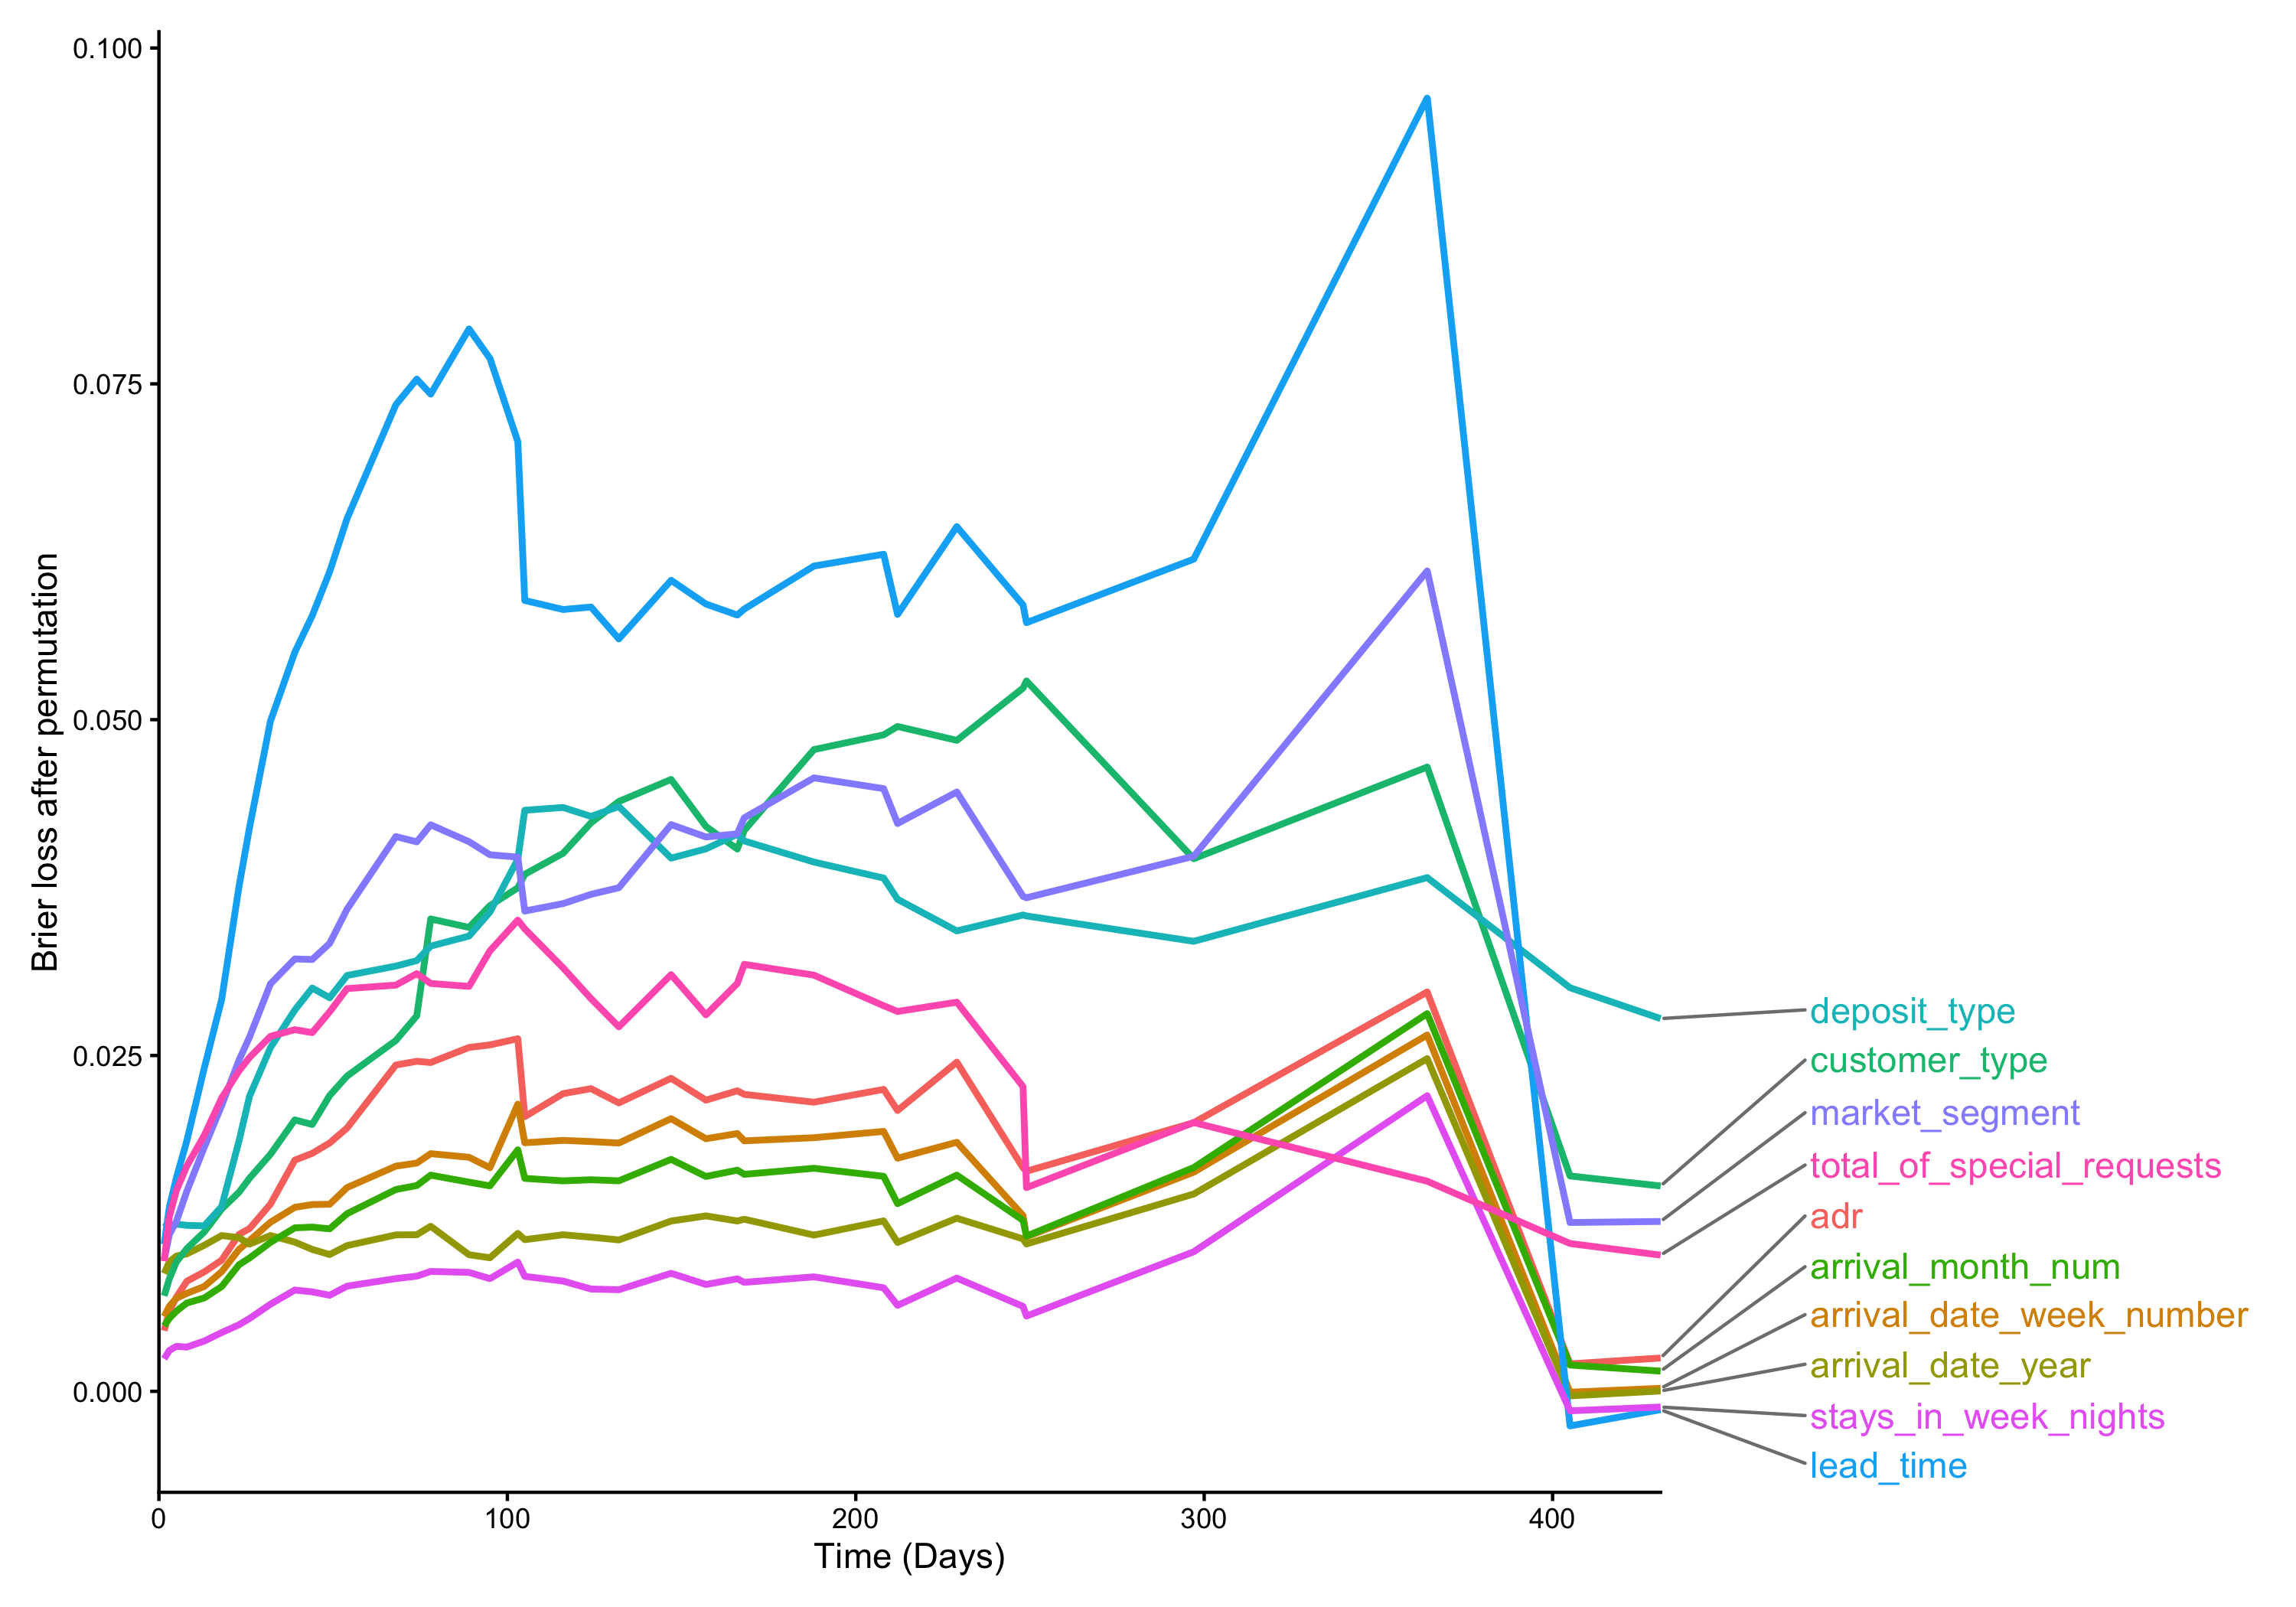
\includegraphics[width=0.88\textwidth]{fig_survpfi_ds1.png}
\caption{Time-dependent Survival Permutation Feature Importance for the Oblique RSF model evaluated on the independent test partition, measured as the delta in Brier loss over time.}\label{fig:survpfi_ds1}
\end{figure*}

While SurvPFI establishes \textit{which} covariates govern predictive performance, it does not reveal the directional marginal effect of these features on the actual non-cancellation survival probability. To evaluate these non-linear functional dependencies, Figure~\ref{fig:survpdp_ds1} presents Partial Dependence Survival Profiles (SurvPDP) across continuous time horizons for the top influential covariates of Oblique RSF.

\begin{figure*}[htbp]
\centering
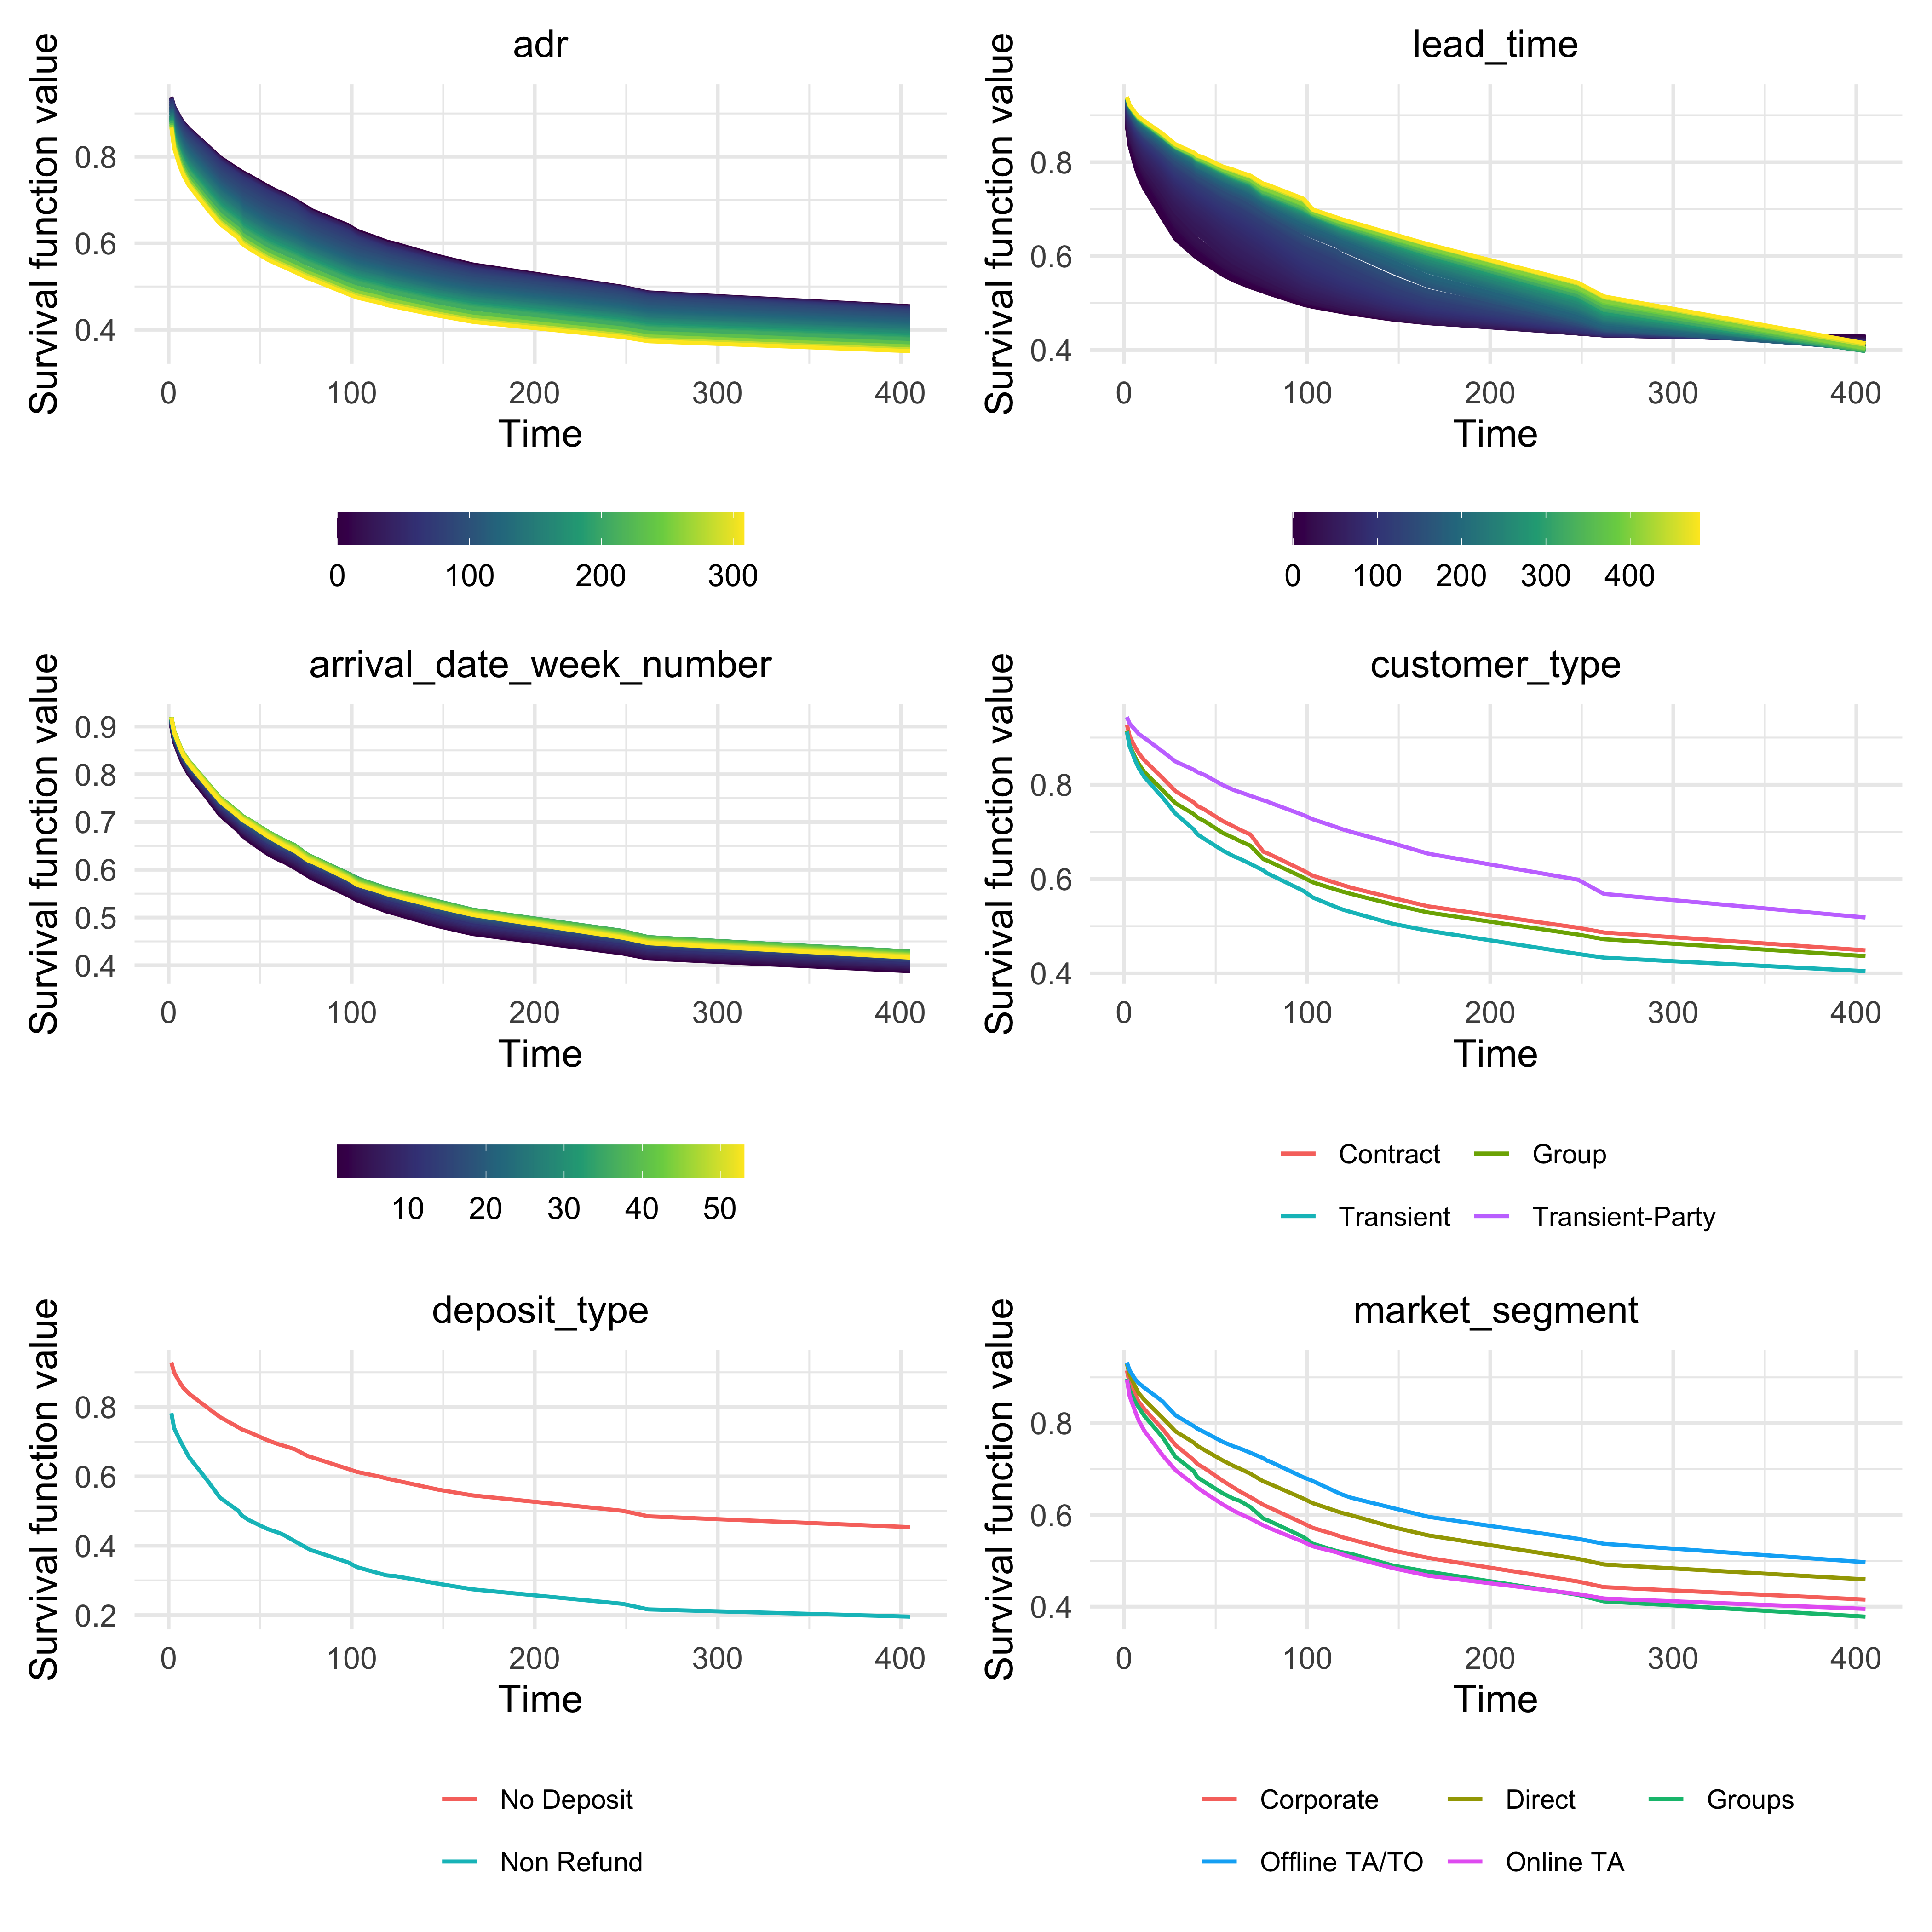
\includegraphics[width=0.92\textwidth]{fig_survpdp_ds1.png}
\caption{Partial Dependence Survival Profiles for the Oblique RSF model. Each panel isolates the marginal effect of a specific feature's values on the non-cancellation survival probability across continuous time.}\label{fig:survpdp_ds1}
\end{figure*}

The SurvPDP profiles illuminate key operational dynamics:
\begin{enumerate}
  \item \textbf{Deposit Type Anomaly}: Bookings categorized with a \textit{Non Refund} policy display a drastically depressed baseline survival probability compared to \textit{No Deposit} reservations. In standard econometric assumptions, non-refundable deposits are intended to enforce contractual commitment; however, in this empirical cohort, non-refundable rates were predominantly applied to speculative group allocations that were subsequently canceled en masse by intermediaries \citep{antonio2019big}. SurvPDP successfully unmasks and isolates this structural anomaly, illustrating the critical role of XAI auditing prior to model deployment.
  \item \textbf{Monotonic Lead Time Decay}: Reservations booked far in advance exhibit a monotonic decline in survival probability, with attrition accelerating noticeably as reservations exceed 100 days.
  \item \textbf{Market Segment Volatility}: Bookings originating from \textit{Groups} and \textit{Online TA} channels maintain consistently lower survival trajectories relative to direct customer bookings, reflecting the low switching costs inherent in digital aggregation platforms.
\end{enumerate}

\section{Discussion}
\label{sec:discussion}

The empirical findings of this study provide critical insights for machine learning methodology, revenue management, and the ethical governance of digital transformation in hospitality.

\subsection{Ethical Implications of Calibrated Predictions for Revenue Management}
In the era of smart hospitality systems, revenue management practices increasingly sit at the intersection of technological optimization and ethical responsibility \citep{law2025ethical}. A central finding of this study is the critical trade-off between rank concordance and probability calibration. While standard Random Survival Forests achieve superior discriminative ordering, their probability calibration is severely distorted, systematically compressing probability estimates. In real-world revenue management, setting overbooking limits based on miscalibrated probabilities directly generates negative ethical externalities: aggressive overbooking driven by distorted attrition forecasts leads to guest denied-boarding/displacement, severe relocation distress, and consumer insecurity \citep{lin2026developing}. By demonstrating that Oblique RSF delivers well-calibrated, continuous probabilities that faithfully track empirical Kaplan-Meier event rates, our framework provides revenue managers with a principled, ethics-by-design mechanism. Calibrated probabilities prevent erratic overbooking, protecting vulnerable travelers while safeguarding property legitimacy.

\subsection{Algorithmic Auditing, Anomaly Detection, and Responsible Governance}
As digital platforms and intelligent intermediaries centralize booking transactions, algorithmic explainability serves as an essential accountability mechanism \citep{dwivedi2025artificial, meske2022explainable}. Rather than treating model explanations as infallible proofs of individual psychology, we demonstrate how time-dependent explainable artificial intelligence functions as a pre-deployment auditing safeguard. The discovery of the \textit{Non Refund} policy anomaly illustrates this ethical dimension: an unaudited black-box model would naively infer that non-refundable reservations inherently carry high cancellation hazards, potentially leading automated systems to penalize legitimate individual travelers who select non-refundable rates. SurvPDP disentangled this anomaly, exposing that the pattern was an artifact of speculative block bookings by intermediaries \citep{antonio2019data}. Continuous explainability therefore operationalizes ethical AI principles by ensuring that automated capacity controls remain auditable, transparent, and fair.

\subsection{Limitations and Future Research}
Several limitations of this study should be acknowledged. First, although our experimental evaluation incorporated 100-replicate non-parametric bootstrap uncertainty estimates, paired Wilcoxon tests, and empirical calibration curves, the evaluation was conducted on a single large-scale empirical cohort with verified timestamps. Future research should evaluate temporal transferability by testing trained models across geographically diverse lodging markets and differing economic cycles. Second, while our analysis leveraged exact event timestamps, all covariates were measured statically at the time of booking. Extending survival frameworks to accommodate time-varying covariates, such as dynamic competitor pricing, macroeconomic sentiment indicators, and local event schedules, through landmark modeling or recurrent neural survival architectures represents a promising avenue for advancing predictive accuracy in revenue management.

\section{Conclusion}
\label{sec:conclusion}

This research introduces an explainable time-to-event predictive modeling framework for hotel booking cancellation forecasting. By framing cancellation as a continuous survival problem with verified right-censoring timestamps, we benchmarked diverse semi-parametric and machine learning survival algorithms across comprehensive evaluation criteria. Through rigorous statistical uncertainty estimation ($B=100$ bootstrap replicates, $95\%$ confidence intervals, and paired hypothesis tests), we demonstrated that while Standard RSF achieves top-tier discriminative concordance, Oblique RSF delivers superior probability calibration and aligns closely with empirical event rates. Furthermore, time-dependent explainable artificial intelligence tools successfully decoded continuous risk dynamics and exposed structural deposit policy anomalies. These findings demonstrate that trustworthy AI in hospitality requires both calibrated probabilities and continuous interpretability, providing hotel revenue managers with a principled foundation for dynamic capacity control and algorithmic governance.

\backmatter

\section*{Declarations}

\textbf{Funding} No funding was received for conducting this study.\\

\noindent \textbf{Competing interests} The author has no competing interests to declare that are relevant to the content of this paper.\\

\noindent \textbf{Author contributions} The author is solely responsible for all aspects of this work, including conceptualization, methodology, formal analysis, investigation, writing, original draft preparation, and writing, review and editing.\\

\noindent \textbf{Data availability} The datasets analysed in this study are publicly available. The Hotel Booking Demand dataset is publicly available at \url{https://doi.org/10.1016/j.dib.2018.11.126}.\\

\noindent \textbf{Code availability} The code for reproducing all experiments is publicly accessible via: \url{https://github.com/mcavs/explainable-hotel-booking-cancellation-predictive-models}.

\bibliography{sn-bibliography}

\end{document}
